% Created by tikzDevice version 0.12.6 on 2026-08-08 12:11:59
% !TEX encoding = UTF-8 Unicode
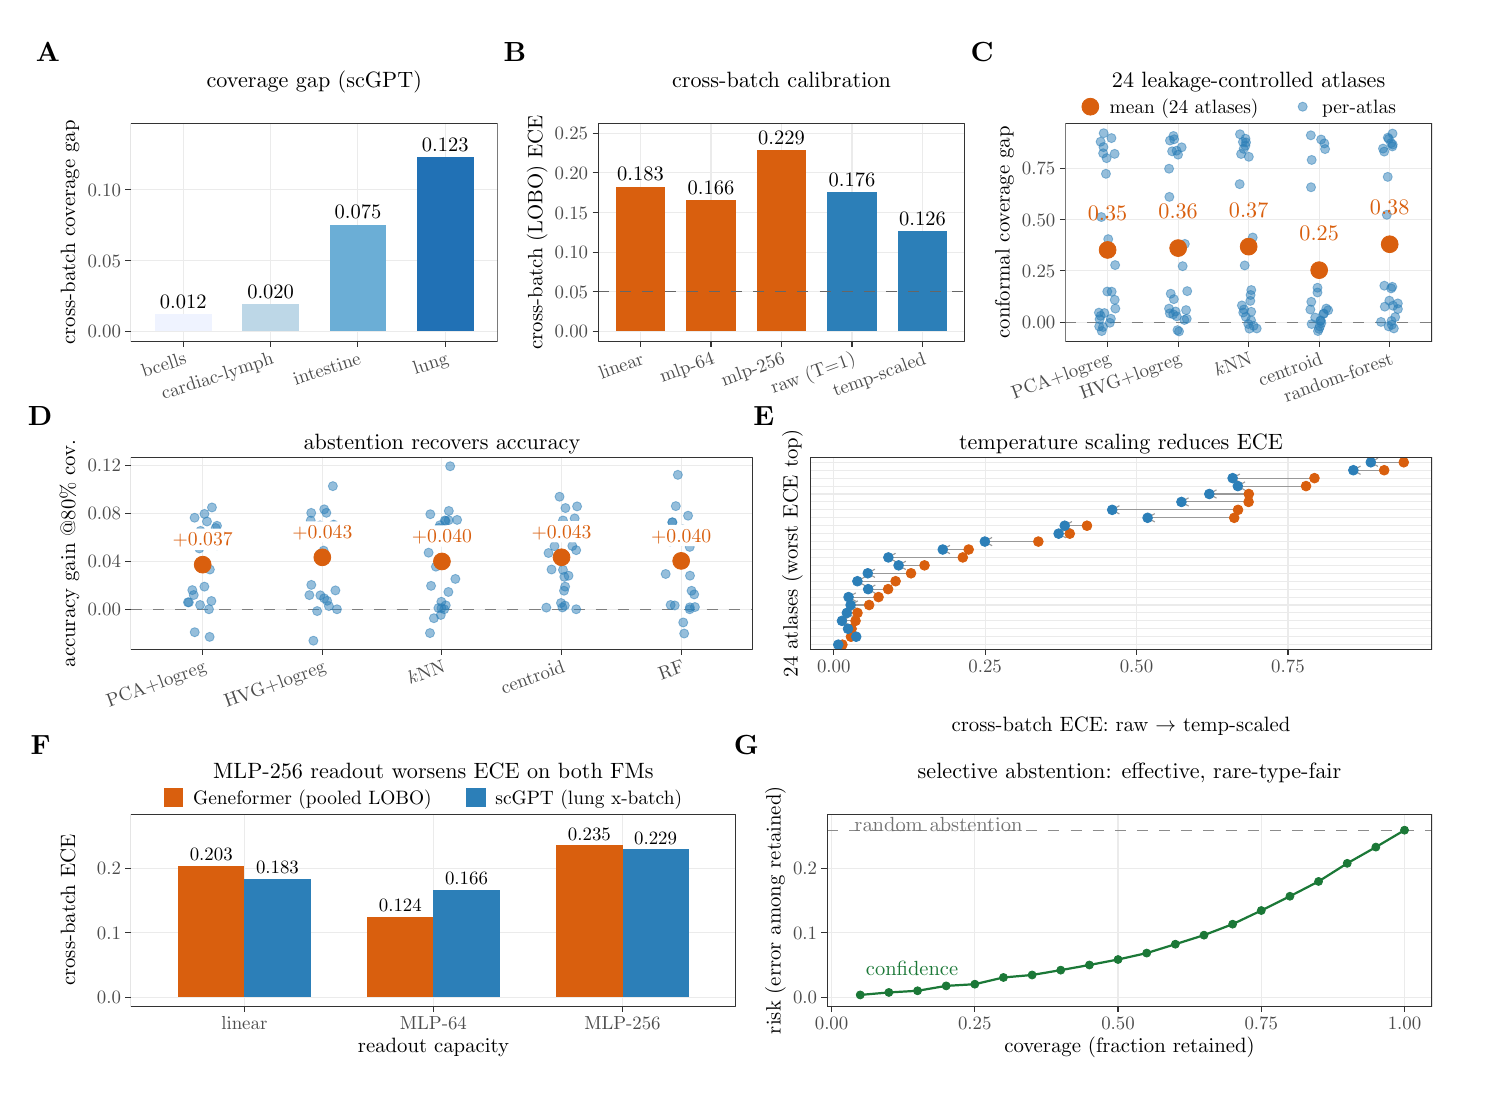
\begin{tikzpicture}[x=1pt,y=1pt]
\definecolor{fillColor}{RGB}{255,255,255}
\path[use as bounding box,fill=fillColor,fill opacity=0.00] (0,0) rectangle (517.45,375.80);
\begin{scope}
\path[clip] (  0.00,  0.00) rectangle (517.45,375.80);
\definecolor{drawColor}{RGB}{255,255,255}
\definecolor{fillColor}{RGB}{255,255,255}

\path[draw=drawColor,line width= 0.4pt,line join=round,line cap=round,fill=fillColor] (  0.00, -0.00) rectangle (517.45,375.80);
\end{scope}
\begin{scope}
\path[clip] (  6.00,237.03) rectangle (174.82,367.80);
\definecolor{drawColor}{RGB}{255,255,255}
\definecolor{fillColor}{RGB}{255,255,255}

\path[draw=drawColor,line width= 0.4pt,line join=round,line cap=round,fill=fillColor] (  6.00,237.03) rectangle (174.82,367.80);
\end{scope}
\begin{scope}
\path[clip] (174.82,237.03) rectangle (343.64,367.80);
\definecolor{drawColor}{RGB}{255,255,255}
\definecolor{fillColor}{RGB}{255,255,255}

\path[draw=drawColor,line width= 0.4pt,line join=round,line cap=round,fill=fillColor] (174.82,237.03) rectangle (343.64,367.80);
\end{scope}
\begin{scope}
\path[clip] (343.64,237.03) rectangle (512.45,367.80);
\definecolor{drawColor}{RGB}{255,255,255}
\definecolor{fillColor}{RGB}{255,255,255}

\path[draw=drawColor,line width= 0.4pt,line join=round,line cap=round,fill=fillColor] (343.64,237.03) rectangle (512.45,367.80);
\end{scope}
\begin{scope}
\path[clip] ( 37.31,262.45) rectangle (169.82,341.24);
\definecolor{fillColor}{RGB}{255,255,255}

\path[fill=fillColor] ( 37.31,262.45) rectangle (169.82,341.24);
\definecolor{drawColor}{gray}{0.92}

\path[draw=drawColor,line width= 0.4pt,line join=round] ( 37.31,266.03) --
	(169.82,266.03);

\path[draw=drawColor,line width= 0.4pt,line join=round] ( 37.31,291.61) --
	(169.82,291.61);

\path[draw=drawColor,line width= 0.4pt,line join=round] ( 37.31,317.19) --
	(169.82,317.19);

\path[draw=drawColor,line width= 0.4pt,line join=round] ( 56.24,262.45) --
	( 56.24,341.24);

\path[draw=drawColor,line width= 0.4pt,line join=round] ( 87.79,262.45) --
	( 87.79,341.24);

\path[draw=drawColor,line width= 0.4pt,line join=round] (119.34,262.45) --
	(119.34,341.24);

\path[draw=drawColor,line width= 0.4pt,line join=round] (150.89,262.45) --
	(150.89,341.24);
\definecolor{fillColor}{RGB}{33,113,181}

\path[fill=fillColor] (140.63,266.03) rectangle (161.14,329.11);
\definecolor{fillColor}{RGB}{239,243,255}

\path[fill=fillColor] ( 45.99,266.03) rectangle ( 66.49,272.37);
\definecolor{fillColor}{RGB}{189,215,231}

\path[fill=fillColor] ( 77.53,266.03) rectangle ( 98.04,276.06);
\definecolor{fillColor}{RGB}{107,174,214}

\path[fill=fillColor] (109.08,266.03) rectangle (129.59,304.66);
\definecolor{drawColor}{RGB}{0,0,0}

\node[text=drawColor,anchor=base,inner sep=0pt, outer sep=0pt, scale=  0.74] at (150.89,331.15) {0.123};

\node[text=drawColor,anchor=base,inner sep=0pt, outer sep=0pt, scale=  0.74] at ( 56.24,274.41) {0.012};

\node[text=drawColor,anchor=base,inner sep=0pt, outer sep=0pt, scale=  0.74] at ( 87.79,278.09) {0.020};

\node[text=drawColor,anchor=base,inner sep=0pt, outer sep=0pt, scale=  0.74] at (119.34,306.69) {0.075};
\definecolor{drawColor}{gray}{0.20}

\path[draw=drawColor,line width= 0.4pt,line join=round,line cap=round] ( 37.31,262.45) rectangle (169.82,341.24);
\end{scope}
\begin{scope}
\path[clip] (  0.00,  0.00) rectangle (517.45,375.80);
\definecolor{drawColor}{gray}{0.30}

\node[text=drawColor,anchor=base east,inner sep=0pt, outer sep=0pt, scale=  0.68] at ( 33.71,263.69) {0.00};

\node[text=drawColor,anchor=base east,inner sep=0pt, outer sep=0pt, scale=  0.68] at ( 33.71,289.27) {0.05};

\node[text=drawColor,anchor=base east,inner sep=0pt, outer sep=0pt, scale=  0.68] at ( 33.71,314.85) {0.10};
\end{scope}
\begin{scope}
\path[clip] (  0.00,  0.00) rectangle (517.45,375.80);
\definecolor{drawColor}{gray}{0.20}

\path[draw=drawColor,line width= 0.4pt,line join=round] ( 35.31,266.03) --
	( 37.31,266.03);

\path[draw=drawColor,line width= 0.4pt,line join=round] ( 35.31,291.61) --
	( 37.31,291.61);

\path[draw=drawColor,line width= 0.4pt,line join=round] ( 35.31,317.19) --
	( 37.31,317.19);
\end{scope}
\begin{scope}
\path[clip] (  0.00,  0.00) rectangle (517.45,375.80);
\definecolor{drawColor}{gray}{0.20}

\path[draw=drawColor,line width= 0.4pt,line join=round] ( 56.24,260.45) --
	( 56.24,262.45);

\path[draw=drawColor,line width= 0.4pt,line join=round] ( 87.79,260.45) --
	( 87.79,262.45);

\path[draw=drawColor,line width= 0.4pt,line join=round] (119.34,260.45) --
	(119.34,262.45);

\path[draw=drawColor,line width= 0.4pt,line join=round] (150.89,260.45) --
	(150.89,262.45);
\end{scope}
\begin{scope}
\path[clip] (  0.00,  0.00) rectangle (517.45,375.80);
\definecolor{drawColor}{gray}{0.30}

\node[text=drawColor,rotate= 18.00,anchor=base east,inner sep=0pt, outer sep=0pt, scale=  0.68] at ( 57.69,254.39) {bcells};

\node[text=drawColor,rotate= 18.00,anchor=base east,inner sep=0pt, outer sep=0pt, scale=  0.68] at ( 89.24,254.39) {cardiac-lymph};

\node[text=drawColor,rotate= 18.00,anchor=base east,inner sep=0pt, outer sep=0pt, scale=  0.68] at (120.79,254.39) {intestine};

\node[text=drawColor,rotate= 18.00,anchor=base east,inner sep=0pt, outer sep=0pt, scale=  0.68] at (152.34,254.39) {lung};
\end{scope}
\begin{scope}
\path[clip] (  0.00,  0.00) rectangle (517.45,375.80);
\definecolor{drawColor}{RGB}{0,0,0}

\node[text=drawColor,rotate= 90.00,anchor=base,inner sep=0pt, outer sep=0pt, scale=  0.75] at ( 17.17,301.84) {cross-batch coverage gap};
\end{scope}
\begin{scope}
\path[clip] (  0.00,  0.00) rectangle (517.45,375.80);
\definecolor{drawColor}{RGB}{0,0,0}

\node[text=drawColor,anchor=base,inner sep=0pt, outer sep=0pt, scale=  0.80] at (103.56,354.29) {coverage gap (scGPT)};
\end{scope}
\begin{scope}
\path[clip] (  0.00,  0.00) rectangle (517.45,375.80);
\definecolor{drawColor}{RGB}{0,0,0}

\node[text=drawColor,anchor=base,inner sep=0pt, outer sep=0pt, scale=  1.00] at (  7.27,363.60) {\bfseries A};
\end{scope}
\begin{scope}
\path[clip] (206.13,262.45) rectangle (338.64,341.24);
\definecolor{fillColor}{RGB}{255,255,255}

\path[fill=fillColor] (206.13,262.45) rectangle (338.64,341.24);
\definecolor{drawColor}{gray}{0.92}

\path[draw=drawColor,line width= 0.4pt,line join=round] (206.13,266.03) --
	(338.64,266.03);

\path[draw=drawColor,line width= 0.4pt,line join=round] (206.13,280.35) --
	(338.64,280.35);

\path[draw=drawColor,line width= 0.4pt,line join=round] (206.13,294.68) --
	(338.64,294.68);

\path[draw=drawColor,line width= 0.4pt,line join=round] (206.13,309.01) --
	(338.64,309.01);

\path[draw=drawColor,line width= 0.4pt,line join=round] (206.13,323.33) --
	(338.64,323.33);

\path[draw=drawColor,line width= 0.4pt,line join=round] (206.13,337.66) --
	(338.64,337.66);

\path[draw=drawColor,line width= 0.4pt,line join=round] (221.42,262.45) --
	(221.42,341.24);

\path[draw=drawColor,line width= 0.4pt,line join=round] (246.90,262.45) --
	(246.90,341.24);

\path[draw=drawColor,line width= 0.4pt,line join=round] (272.38,262.45) --
	(272.38,341.24);

\path[draw=drawColor,line width= 0.4pt,line join=round] (297.86,262.45) --
	(297.86,341.24);

\path[draw=drawColor,line width= 0.4pt,line join=round] (323.35,262.45) --
	(323.35,341.24);
\definecolor{fillColor}{RGB}{217,95,14}

\path[fill=fillColor] (212.50,266.03) rectangle (230.34,318.40);

\path[fill=fillColor] (237.98,266.03) rectangle (255.82,313.53);

\path[fill=fillColor] (263.46,266.03) rectangle (281.30,331.67);
\definecolor{fillColor}{RGB}{44,127,184}

\path[fill=fillColor] (288.94,266.03) rectangle (306.78,316.51);

\path[fill=fillColor] (314.43,266.03) rectangle (332.26,302.19);
\definecolor{drawColor}{RGB}{0,0,0}

\node[text=drawColor,anchor=base,inner sep=0pt, outer sep=0pt, scale=  0.74] at (221.42,320.44) {0.183};

\node[text=drawColor,anchor=base,inner sep=0pt, outer sep=0pt, scale=  0.74] at (246.90,315.57) {0.166};

\node[text=drawColor,anchor=base,inner sep=0pt, outer sep=0pt, scale=  0.74] at (272.38,333.71) {0.229};

\node[text=drawColor,anchor=base,inner sep=0pt, outer sep=0pt, scale=  0.74] at (297.86,318.55) {0.176};

\node[text=drawColor,anchor=base,inner sep=0pt, outer sep=0pt, scale=  0.74] at (323.35,304.22) {0.126};
\definecolor{drawColor}{gray}{0.40}

\path[draw=drawColor,line width= 0.4pt,dash pattern=on 4pt off 4pt ,line join=round] (206.13,280.35) -- (338.64,280.35);
\definecolor{drawColor}{gray}{0.20}

\path[draw=drawColor,line width= 0.4pt,line join=round,line cap=round] (206.13,262.45) rectangle (338.64,341.24);
\end{scope}
\begin{scope}
\path[clip] (  0.00,  0.00) rectangle (517.45,375.80);
\definecolor{drawColor}{gray}{0.30}

\node[text=drawColor,anchor=base east,inner sep=0pt, outer sep=0pt, scale=  0.68] at (202.53,263.69) {0.00};

\node[text=drawColor,anchor=base east,inner sep=0pt, outer sep=0pt, scale=  0.68] at (202.53,278.01) {0.05};

\node[text=drawColor,anchor=base east,inner sep=0pt, outer sep=0pt, scale=  0.68] at (202.53,292.34) {0.10};

\node[text=drawColor,anchor=base east,inner sep=0pt, outer sep=0pt, scale=  0.68] at (202.53,306.66) {0.15};

\node[text=drawColor,anchor=base east,inner sep=0pt, outer sep=0pt, scale=  0.68] at (202.53,320.99) {0.20};

\node[text=drawColor,anchor=base east,inner sep=0pt, outer sep=0pt, scale=  0.68] at (202.53,335.32) {0.25};
\end{scope}
\begin{scope}
\path[clip] (  0.00,  0.00) rectangle (517.45,375.80);
\definecolor{drawColor}{gray}{0.20}

\path[draw=drawColor,line width= 0.4pt,line join=round] (204.13,266.03) --
	(206.13,266.03);

\path[draw=drawColor,line width= 0.4pt,line join=round] (204.13,280.35) --
	(206.13,280.35);

\path[draw=drawColor,line width= 0.4pt,line join=round] (204.13,294.68) --
	(206.13,294.68);

\path[draw=drawColor,line width= 0.4pt,line join=round] (204.13,309.01) --
	(206.13,309.01);

\path[draw=drawColor,line width= 0.4pt,line join=round] (204.13,323.33) --
	(206.13,323.33);

\path[draw=drawColor,line width= 0.4pt,line join=round] (204.13,337.66) --
	(206.13,337.66);
\end{scope}
\begin{scope}
\path[clip] (  0.00,  0.00) rectangle (517.45,375.80);
\definecolor{drawColor}{gray}{0.20}

\path[draw=drawColor,line width= 0.4pt,line join=round] (221.42,260.45) --
	(221.42,262.45);

\path[draw=drawColor,line width= 0.4pt,line join=round] (246.90,260.45) --
	(246.90,262.45);

\path[draw=drawColor,line width= 0.4pt,line join=round] (272.38,260.45) --
	(272.38,262.45);

\path[draw=drawColor,line width= 0.4pt,line join=round] (297.86,260.45) --
	(297.86,262.45);

\path[draw=drawColor,line width= 0.4pt,line join=round] (323.35,260.45) --
	(323.35,262.45);
\end{scope}
\begin{scope}
\path[clip] (  0.00,  0.00) rectangle (517.45,375.80);
\definecolor{drawColor}{gray}{0.30}

\node[text=drawColor,rotate= 20.00,anchor=base east,inner sep=0pt, outer sep=0pt, scale=  0.68] at (223.02,254.45) {linear};

\node[text=drawColor,rotate= 20.00,anchor=base east,inner sep=0pt, outer sep=0pt, scale=  0.68] at (248.50,254.45) {mlp-64};

\node[text=drawColor,rotate= 20.00,anchor=base east,inner sep=0pt, outer sep=0pt, scale=  0.68] at (273.98,254.45) {mlp-256};

\node[text=drawColor,rotate= 20.00,anchor=base east,inner sep=0pt, outer sep=0pt, scale=  0.68] at (299.47,254.45) {raw (T=1)};

\node[text=drawColor,rotate= 20.00,anchor=base east,inner sep=0pt, outer sep=0pt, scale=  0.68] at (324.95,254.45) {temp-scaled};
\end{scope}
\begin{scope}
\path[clip] (  0.00,  0.00) rectangle (517.45,375.80);
\definecolor{drawColor}{RGB}{0,0,0}

\node[text=drawColor,rotate= 90.00,anchor=base,inner sep=0pt, outer sep=0pt, scale=  0.75] at (185.98,301.84) {cross-batch (LOBO) ECE};
\end{scope}
\begin{scope}
\path[clip] (  0.00,  0.00) rectangle (517.45,375.80);
\definecolor{drawColor}{RGB}{0,0,0}

\node[text=drawColor,anchor=base,inner sep=0pt, outer sep=0pt, scale=  0.80] at (272.38,354.29) {cross-batch calibration};
\end{scope}
\begin{scope}
\path[clip] (  0.00,  0.00) rectangle (517.45,375.80);
\definecolor{drawColor}{RGB}{0,0,0}

\node[text=drawColor,anchor=base,inner sep=0pt, outer sep=0pt, scale=  1.00] at (176.08,363.60) {\bfseries B};
\end{scope}
\begin{scope}
\path[clip] (374.94,262.45) rectangle (507.45,341.24);
\definecolor{fillColor}{RGB}{255,255,255}

\path[fill=fillColor] (374.94,262.45) rectangle (507.45,341.24);
\definecolor{drawColor}{gray}{0.92}

\path[draw=drawColor,line width= 0.4pt,line join=round] (374.94,269.39) --
	(507.45,269.39);

\path[draw=drawColor,line width= 0.4pt,line join=round] (374.94,287.91) --
	(507.45,287.91);

\path[draw=drawColor,line width= 0.4pt,line join=round] (374.94,306.43) --
	(507.45,306.43);

\path[draw=drawColor,line width= 0.4pt,line join=round] (374.94,324.95) --
	(507.45,324.95);

\path[draw=drawColor,line width= 0.4pt,line join=round] (390.23,262.45) --
	(390.23,341.24);

\path[draw=drawColor,line width= 0.4pt,line join=round] (415.72,262.45) --
	(415.72,341.24);

\path[draw=drawColor,line width= 0.4pt,line join=round] (441.20,262.45) --
	(441.20,341.24);

\path[draw=drawColor,line width= 0.4pt,line join=round] (466.68,262.45) --
	(466.68,341.24);

\path[draw=drawColor,line width= 0.4pt,line join=round] (492.16,262.45) --
	(492.16,341.24);
\definecolor{drawColor}{gray}{0.50}

\path[draw=drawColor,line width= 0.4pt,dash pattern=on 4pt off 4pt ,line join=round] (374.94,269.39) -- (507.45,269.39);
\definecolor{drawColor}{RGB}{44,127,184}
\definecolor{fillColor}{RGB}{44,127,184}

\path[draw=drawColor,draw opacity=0.50,line width= 0.3pt,line join=round,line cap=round,fill=fillColor,fill opacity=0.50] (388.73,332.65) circle (  1.65);

\path[draw=drawColor,draw opacity=0.50,line width= 0.3pt,line join=round,line cap=round,fill=fillColor,fill opacity=0.50] (416.99,332.56) circle (  1.65);

\path[draw=drawColor,draw opacity=0.50,line width= 0.3pt,line join=round,line cap=round,fill=fillColor,fill opacity=0.50] (440.02,333.14) circle (  1.65);

\path[draw=drawColor,draw opacity=0.50,line width= 0.3pt,line join=round,line cap=round,fill=fillColor,fill opacity=0.50] (463.97,328.00) circle (  1.65);

\path[draw=drawColor,draw opacity=0.50,line width= 0.3pt,line join=round,line cap=round,fill=fillColor,fill opacity=0.50] (493.25,333.56) circle (  1.65);

\path[draw=drawColor,draw opacity=0.50,line width= 0.3pt,line join=round,line cap=round,fill=fillColor,fill opacity=0.50] (392.77,330.20) circle (  1.65);

\path[draw=drawColor,draw opacity=0.50,line width= 0.3pt,line join=round,line cap=round,fill=fillColor,fill opacity=0.50] (415.15,331.34) circle (  1.65);

\path[draw=drawColor,draw opacity=0.50,line width= 0.3pt,line join=round,line cap=round,fill=fillColor,fill opacity=0.50] (439.40,332.01) circle (  1.65);

\path[draw=drawColor,draw opacity=0.50,line width= 0.3pt,line join=round,line cap=round,fill=fillColor,fill opacity=0.50] (468.81,331.93) circle (  1.65);

\path[draw=drawColor,draw opacity=0.50,line width= 0.3pt,line join=round,line cap=round,fill=fillColor,fill opacity=0.50] (490.18,331.02) circle (  1.65);

\path[draw=drawColor,draw opacity=0.50,line width= 0.3pt,line join=round,line cap=round,fill=fillColor,fill opacity=0.50] (387.96,307.37) circle (  1.65);

\path[draw=drawColor,draw opacity=0.50,line width= 0.3pt,line join=round,line cap=round,fill=fillColor,fill opacity=0.50] (412.55,314.65) circle (  1.65);

\path[draw=drawColor,draw opacity=0.50,line width= 0.3pt,line join=round,line cap=round,fill=fillColor,fill opacity=0.50] (437.95,319.26) circle (  1.65);

\path[draw=drawColor,draw opacity=0.50,line width= 0.3pt,line join=round,line cap=round,fill=fillColor,fill opacity=0.50] (469.26,274.30) circle (  1.65);

\path[draw=drawColor,draw opacity=0.50,line width= 0.3pt,line join=round,line cap=round,fill=fillColor,fill opacity=0.50] (491.45,321.88) circle (  1.65);

\path[draw=drawColor,draw opacity=0.50,line width= 0.3pt,line join=round,line cap=round,fill=fillColor,fill opacity=0.50] (388.58,267.64) circle (  1.65);

\path[draw=drawColor,draw opacity=0.50,line width= 0.3pt,line join=round,line cap=round,fill=fillColor,fill opacity=0.50] (415.47,266.50) circle (  1.65);

\path[draw=drawColor,draw opacity=0.50,line width= 0.3pt,line join=round,line cap=round,fill=fillColor,fill opacity=0.50] (442.98,268.06) circle (  1.65);

\path[draw=drawColor,draw opacity=0.50,line width= 0.3pt,line join=round,line cap=round,fill=fillColor,fill opacity=0.50] (466.24,266.17) circle (  1.65);

\path[draw=drawColor,draw opacity=0.50,line width= 0.3pt,line join=round,line cap=round,fill=fillColor,fill opacity=0.50] (491.77,267.86) circle (  1.65);

\path[draw=drawColor,draw opacity=0.50,line width= 0.3pt,line join=round,line cap=round,fill=fillColor,fill opacity=0.50] (387.34,270.45) circle (  1.65);

\path[draw=drawColor,draw opacity=0.50,line width= 0.3pt,line join=round,line cap=round,fill=fillColor,fill opacity=0.50] (413.96,272.21) circle (  1.65);

\path[draw=drawColor,draw opacity=0.50,line width= 0.3pt,line join=round,line cap=round,fill=fillColor,fill opacity=0.50] (439.51,273.97) circle (  1.65);

\path[draw=drawColor,draw opacity=0.50,line width= 0.3pt,line join=round,line cap=round,fill=fillColor,fill opacity=0.50] (468.22,272.37) circle (  1.65);

\path[draw=drawColor,draw opacity=0.50,line width= 0.3pt,line join=round,line cap=round,fill=fillColor,fill opacity=0.50] (492.04,277.16) circle (  1.65);

\path[draw=drawColor,draw opacity=0.50,line width= 0.3pt,line join=round,line cap=round,fill=fillColor,fill opacity=0.50] (391.62,335.90) circle (  1.65);

\path[draw=drawColor,draw opacity=0.50,line width= 0.3pt,line join=round,line cap=round,fill=fillColor,fill opacity=0.50] (414.28,335.47) circle (  1.65);

\path[draw=drawColor,draw opacity=0.50,line width= 0.3pt,line join=round,line cap=round,fill=fillColor,fill opacity=0.50] (440.06,335.67) circle (  1.65);

\path[draw=drawColor,draw opacity=0.50,line width= 0.3pt,line join=round,line cap=round,fill=fillColor,fill opacity=0.50] (468.55,333.97) circle (  1.65);

\path[draw=drawColor,draw opacity=0.50,line width= 0.3pt,line join=round,line cap=round,fill=fillColor,fill opacity=0.50] (491.48,336.04) circle (  1.65);

\path[draw=drawColor,draw opacity=0.50,line width= 0.3pt,line join=round,line cap=round,fill=fillColor,fill opacity=0.50] (390.45,299.38) circle (  1.65);

\path[draw=drawColor,draw opacity=0.50,line width= 0.3pt,line join=round,line cap=round,fill=fillColor,fill opacity=0.50] (418.14,297.65) circle (  1.65);

\path[draw=drawColor,draw opacity=0.50,line width= 0.3pt,line join=round,line cap=round,fill=fillColor,fill opacity=0.50] (442.67,299.97) circle (  1.65);

\path[draw=drawColor,draw opacity=0.50,line width= 0.3pt,line join=round,line cap=round,fill=fillColor,fill opacity=0.50] (466.37,288.13) circle (  1.65);

\path[draw=drawColor,draw opacity=0.50,line width= 0.3pt,line join=round,line cap=round,fill=fillColor,fill opacity=0.50] (491.12,308.18) circle (  1.65);

\path[draw=drawColor,draw opacity=0.50,line width= 0.3pt,line join=round,line cap=round,fill=fillColor,fill opacity=0.50] (387.70,334.58) circle (  1.65);

\path[draw=drawColor,draw opacity=0.50,line width= 0.3pt,line join=round,line cap=round,fill=fillColor,fill opacity=0.50] (412.76,335.01) circle (  1.65);

\path[draw=drawColor,draw opacity=0.50,line width= 0.3pt,line join=round,line cap=round,fill=fillColor,fill opacity=0.50] (440.25,334.33) circle (  1.65);

\path[draw=drawColor,draw opacity=0.50,line width= 0.3pt,line join=round,line cap=round,fill=fillColor,fill opacity=0.50] (467.39,335.38) circle (  1.65);

\path[draw=drawColor,draw opacity=0.50,line width= 0.3pt,line join=round,line cap=round,fill=fillColor,fill opacity=0.50] (492.68,334.08) circle (  1.65);

\path[draw=drawColor,draw opacity=0.50,line width= 0.3pt,line join=round,line cap=round,fill=fillColor,fill opacity=0.50] (391.41,270.62) circle (  1.65);

\path[draw=drawColor,draw opacity=0.50,line width= 0.3pt,line join=round,line cap=round,fill=fillColor,fill opacity=0.50] (417.35,289.61) circle (  1.65);

\path[draw=drawColor,draw opacity=0.50,line width= 0.3pt,line join=round,line cap=round,fill=fillColor,fill opacity=0.50] (439.77,289.88) circle (  1.65);

\path[draw=drawColor,draw opacity=0.50,line width= 0.3pt,line join=round,line cap=round,fill=fillColor,fill opacity=0.50] (466.07,281.82) circle (  1.65);

\path[draw=drawColor,draw opacity=0.50,line width= 0.3pt,line join=round,line cap=round,fill=fillColor,fill opacity=0.50] (493.11,282.16) circle (  1.65);

\path[draw=drawColor,draw opacity=0.50,line width= 0.3pt,line join=round,line cap=round,fill=fillColor,fill opacity=0.50] (391.70,280.40) circle (  1.65);

\path[draw=drawColor,draw opacity=0.50,line width= 0.3pt,line join=round,line cap=round,fill=fillColor,fill opacity=0.50] (419.00,280.59) circle (  1.65);

\path[draw=drawColor,draw opacity=0.50,line width= 0.3pt,line join=round,line cap=round,fill=fillColor,fill opacity=0.50] (441.89,279.20) circle (  1.65);

\path[draw=drawColor,draw opacity=0.50,line width= 0.3pt,line join=round,line cap=round,fill=fillColor,fill opacity=0.50] (466.06,280.11) circle (  1.65);

\path[draw=drawColor,draw opacity=0.50,line width= 0.3pt,line join=round,line cap=round,fill=fillColor,fill opacity=0.50] (490.23,282.56) circle (  1.65);

\path[draw=drawColor,draw opacity=0.50,line width= 0.3pt,line join=round,line cap=round,fill=fillColor,fill opacity=0.50] (388.11,266.17) circle (  1.65);

\path[draw=drawColor,draw opacity=0.50,line width= 0.3pt,line join=round,line cap=round,fill=fillColor,fill opacity=0.50] (416.04,266.03) circle (  1.65);

\path[draw=drawColor,draw opacity=0.50,line width= 0.3pt,line join=round,line cap=round,fill=fillColor,fill opacity=0.50] (441.49,267.05) circle (  1.65);

\path[draw=drawColor,draw opacity=0.50,line width= 0.3pt,line join=round,line cap=round,fill=fillColor,fill opacity=0.50] (467.46,269.08) circle (  1.65);

\path[draw=drawColor,draw opacity=0.50,line width= 0.3pt,line join=round,line cap=round,fill=fillColor,fill opacity=0.50] (493.65,267.12) circle (  1.65);

\path[draw=drawColor,draw opacity=0.50,line width= 0.3pt,line join=round,line cap=round,fill=fillColor,fill opacity=0.50] (390.12,280.46) circle (  1.65);

\path[draw=drawColor,draw opacity=0.50,line width= 0.3pt,line join=round,line cap=round,fill=fillColor,fill opacity=0.50] (413.04,279.66) circle (  1.65);

\path[draw=drawColor,draw opacity=0.50,line width= 0.3pt,line join=round,line cap=round,fill=fillColor,fill opacity=0.50] (442.12,273.13) circle (  1.65);

\path[draw=drawColor,draw opacity=0.50,line width= 0.3pt,line join=round,line cap=round,fill=fillColor,fill opacity=0.50] (468.35,272.51) circle (  1.65);

\path[draw=drawColor,draw opacity=0.50,line width= 0.3pt,line join=round,line cap=round,fill=fillColor,fill opacity=0.50] (493.37,275.31) circle (  1.65);

\path[draw=drawColor,draw opacity=0.50,line width= 0.3pt,line join=round,line cap=round,fill=fillColor,fill opacity=0.50] (388.81,337.66) circle (  1.65);

\path[draw=drawColor,draw opacity=0.50,line width= 0.3pt,line join=round,line cap=round,fill=fillColor,fill opacity=0.50] (414.02,336.65) circle (  1.65);

\path[draw=drawColor,draw opacity=0.50,line width= 0.3pt,line join=round,line cap=round,fill=fillColor,fill opacity=0.50] (438.06,337.28) circle (  1.65);

\path[draw=drawColor,draw opacity=0.50,line width= 0.3pt,line join=round,line cap=round,fill=fillColor,fill opacity=0.50] (463.66,336.90) circle (  1.65);

\path[draw=drawColor,draw opacity=0.50,line width= 0.3pt,line join=round,line cap=round,fill=fillColor,fill opacity=0.50] (493.19,337.53) circle (  1.65);

\path[draw=drawColor,draw opacity=0.50,line width= 0.3pt,line join=round,line cap=round,fill=fillColor,fill opacity=0.50] (392.95,290.01) circle (  1.65);

\path[draw=drawColor,draw opacity=0.50,line width= 0.3pt,line join=round,line cap=round,fill=fillColor,fill opacity=0.50] (412.74,272.57) circle (  1.65);

\path[draw=drawColor,draw opacity=0.50,line width= 0.3pt,line join=round,line cap=round,fill=fillColor,fill opacity=0.50] (438.76,275.43) circle (  1.65);

\path[draw=drawColor,draw opacity=0.50,line width= 0.3pt,line join=round,line cap=round,fill=fillColor,fill opacity=0.50] (466.06,288.40) circle (  1.65);

\path[draw=drawColor,draw opacity=0.50,line width= 0.3pt,line join=round,line cap=round,fill=fillColor,fill opacity=0.50] (492.69,281.58) circle (  1.65);

\path[draw=drawColor,draw opacity=0.50,line width= 0.3pt,line join=round,line cap=round,fill=fillColor,fill opacity=0.50] (391.03,269.16) circle (  1.65);

\path[draw=drawColor,draw opacity=0.50,line width= 0.3pt,line join=round,line cap=round,fill=fillColor,fill opacity=0.50] (418.83,270.61) circle (  1.65);

\path[draw=drawColor,draw opacity=0.50,line width= 0.3pt,line join=round,line cap=round,fill=fillColor,fill opacity=0.50] (441.05,268.73) circle (  1.65);

\path[draw=drawColor,draw opacity=0.50,line width= 0.3pt,line join=round,line cap=round,fill=fillColor,fill opacity=0.50] (463.96,268.70) circle (  1.65);

\path[draw=drawColor,draw opacity=0.50,line width= 0.3pt,line join=round,line cap=round,fill=fillColor,fill opacity=0.50] (492.82,269.80) circle (  1.65);

\path[draw=drawColor,draw opacity=0.50,line width= 0.3pt,line join=round,line cap=round,fill=fillColor,fill opacity=0.50] (387.19,267.86) circle (  1.65);

\path[draw=drawColor,draw opacity=0.50,line width= 0.3pt,line join=round,line cap=round,fill=fillColor,fill opacity=0.50] (417.96,270.17) circle (  1.65);

\path[draw=drawColor,draw opacity=0.50,line width= 0.3pt,line join=round,line cap=round,fill=fillColor,fill opacity=0.50] (442.07,270.06) circle (  1.65);

\path[draw=drawColor,draw opacity=0.50,line width= 0.3pt,line join=round,line cap=round,fill=fillColor,fill opacity=0.50] (467.09,269.85) circle (  1.65);

\path[draw=drawColor,draw opacity=0.50,line width= 0.3pt,line join=round,line cap=round,fill=fillColor,fill opacity=0.50] (489.02,269.47) circle (  1.65);

\path[draw=drawColor,draw opacity=0.50,line width= 0.3pt,line join=round,line cap=round,fill=fillColor,fill opacity=0.50] (389.85,328.64) circle (  1.65);

\path[draw=drawColor,draw opacity=0.50,line width= 0.3pt,line join=round,line cap=round,fill=fillColor,fill opacity=0.50] (415.68,329.92) circle (  1.65);

\path[draw=drawColor,draw opacity=0.50,line width= 0.3pt,line join=round,line cap=round,fill=fillColor,fill opacity=0.50] (441.26,329.14) circle (  1.65);

\path[draw=drawColor,draw opacity=0.50,line width= 0.3pt,line join=round,line cap=round,fill=fillColor,fill opacity=0.50] (463.84,276.74) circle (  1.65);

\path[draw=drawColor,draw opacity=0.50,line width= 0.3pt,line join=round,line cap=round,fill=fillColor,fill opacity=0.50] (489.74,332.11) circle (  1.65);

\path[draw=drawColor,draw opacity=0.50,line width= 0.3pt,line join=round,line cap=round,fill=fillColor,fill opacity=0.50] (392.80,277.45) circle (  1.65);

\path[draw=drawColor,draw opacity=0.50,line width= 0.3pt,line join=round,line cap=round,fill=fillColor,fill opacity=0.50] (414.16,277.69) circle (  1.65);

\path[draw=drawColor,draw opacity=0.50,line width= 0.3pt,line join=round,line cap=round,fill=fillColor,fill opacity=0.50] (442.15,280.99) circle (  1.65);

\path[draw=drawColor,draw opacity=0.50,line width= 0.3pt,line join=round,line cap=round,fill=fillColor,fill opacity=0.50] (466.96,267.83) circle (  1.65);

\path[draw=drawColor,draw opacity=0.50,line width= 0.3pt,line join=round,line cap=round,fill=fillColor,fill opacity=0.50] (490.39,274.99) circle (  1.65);

\path[draw=drawColor,draw opacity=0.50,line width= 0.3pt,line join=round,line cap=round,fill=fillColor,fill opacity=0.50] (389.08,272.68) circle (  1.65);

\path[draw=drawColor,draw opacity=0.50,line width= 0.3pt,line join=round,line cap=round,fill=fillColor,fill opacity=0.50] (414.78,273.24) circle (  1.65);

\path[draw=drawColor,draw opacity=0.50,line width= 0.3pt,line join=round,line cap=round,fill=fillColor,fill opacity=0.50] (439.24,272.87) circle (  1.65);

\path[draw=drawColor,draw opacity=0.50,line width= 0.3pt,line join=round,line cap=round,fill=fillColor,fill opacity=0.50] (463.50,273.95) circle (  1.65);

\path[draw=drawColor,draw opacity=0.50,line width= 0.3pt,line join=round,line cap=round,fill=fillColor,fill opacity=0.50] (495.13,274.13) circle (  1.65);

\path[draw=drawColor,draw opacity=0.50,line width= 0.3pt,line join=round,line cap=round,fill=fillColor,fill opacity=0.50] (389.63,322.99) circle (  1.65);

\path[draw=drawColor,draw opacity=0.50,line width= 0.3pt,line join=round,line cap=round,fill=fillColor,fill opacity=0.50] (412.44,324.83) circle (  1.65);

\path[draw=drawColor,draw opacity=0.50,line width= 0.3pt,line join=round,line cap=round,fill=fillColor,fill opacity=0.50] (438.46,330.15) circle (  1.65);

\path[draw=drawColor,draw opacity=0.50,line width= 0.3pt,line join=round,line cap=round,fill=fillColor,fill opacity=0.50] (463.74,318.13) circle (  1.65);

\path[draw=drawColor,draw opacity=0.50,line width= 0.3pt,line join=round,line cap=round,fill=fillColor,fill opacity=0.50] (493.13,332.88) circle (  1.65);

\path[draw=drawColor,draw opacity=0.50,line width= 0.3pt,line join=round,line cap=round,fill=fillColor,fill opacity=0.50] (393.03,274.30) circle (  1.65);

\path[draw=drawColor,draw opacity=0.50,line width= 0.3pt,line join=round,line cap=round,fill=fillColor,fill opacity=0.50] (418.58,273.74) circle (  1.65);

\path[draw=drawColor,draw opacity=0.50,line width= 0.3pt,line join=round,line cap=round,fill=fillColor,fill opacity=0.50] (440.16,271.29) circle (  1.65);

\path[draw=drawColor,draw opacity=0.50,line width= 0.3pt,line join=round,line cap=round,fill=fillColor,fill opacity=0.50] (465.24,271.05) circle (  1.65);

\path[draw=drawColor,draw opacity=0.50,line width= 0.3pt,line join=round,line cap=round,fill=fillColor,fill opacity=0.50] (494.15,271.21) circle (  1.65);

\path[draw=drawColor,draw opacity=0.50,line width= 0.3pt,line join=round,line cap=round,fill=fillColor,fill opacity=0.50] (387.09,272.82) circle (  1.65);

\path[draw=drawColor,draw opacity=0.50,line width= 0.3pt,line join=round,line cap=round,fill=fillColor,fill opacity=0.50] (415.21,271.48) circle (  1.65);

\path[draw=drawColor,draw opacity=0.50,line width= 0.3pt,line join=round,line cap=round,fill=fillColor,fill opacity=0.50] (444.11,267.10) circle (  1.65);

\path[draw=drawColor,draw opacity=0.50,line width= 0.3pt,line join=round,line cap=round,fill=fillColor,fill opacity=0.50] (466.62,266.97) circle (  1.65);

\path[draw=drawColor,draw opacity=0.50,line width= 0.3pt,line join=round,line cap=round,fill=fillColor,fill opacity=0.50] (492.92,268.43) circle (  1.65);

\path[draw=drawColor,draw opacity=0.50,line width= 0.3pt,line join=round,line cap=round,fill=fillColor,fill opacity=0.50] (387.72,271.67) circle (  1.65);

\path[draw=drawColor,draw opacity=0.50,line width= 0.3pt,line join=round,line cap=round,fill=fillColor,fill opacity=0.50] (412.42,274.27) circle (  1.65);

\path[draw=drawColor,draw opacity=0.50,line width= 0.3pt,line join=round,line cap=round,fill=fillColor,fill opacity=0.50] (441.80,277.07) circle (  1.65);

\path[draw=drawColor,draw opacity=0.50,line width= 0.3pt,line join=round,line cap=round,fill=fillColor,fill opacity=0.50] (469.94,273.70) circle (  1.65);

\path[draw=drawColor,draw opacity=0.50,line width= 0.3pt,line join=round,line cap=round,fill=fillColor,fill opacity=0.50] (495.10,276.15) circle (  1.65);

\path[draw=drawColor,draw opacity=0.50,line width= 0.3pt,line join=round,line cap=round,fill=fillColor,fill opacity=0.50] (388.61,330.40) circle (  1.65);

\path[draw=drawColor,draw opacity=0.50,line width= 0.3pt,line join=round,line cap=round,fill=fillColor,fill opacity=0.50] (413.54,331.12) circle (  1.65);

\path[draw=drawColor,draw opacity=0.50,line width= 0.3pt,line join=round,line cap=round,fill=fillColor,fill opacity=0.50] (439.11,334.50) circle (  1.65);

\path[draw=drawColor,draw opacity=0.50,line width= 0.3pt,line join=round,line cap=round,fill=fillColor,fill opacity=0.50] (467.27,270.01) circle (  1.65);

\path[draw=drawColor,draw opacity=0.50,line width= 0.3pt,line join=round,line cap=round,fill=fillColor,fill opacity=0.50] (491.84,335.63) circle (  1.65);
\definecolor{drawColor}{RGB}{217,95,14}
\definecolor{fillColor}{RGB}{217,95,14}

\path[draw=drawColor,line width= 0.3pt,line join=round,line cap=round,fill=fillColor] (390.23,295.48) circle (  3.04);

\path[draw=drawColor,line width= 0.3pt,line join=round,line cap=round,fill=fillColor] (415.72,296.15) circle (  3.04);

\path[draw=drawColor,line width= 0.3pt,line join=round,line cap=round,fill=fillColor] (441.20,296.68) circle (  3.04);

\path[draw=drawColor,line width= 0.3pt,line join=round,line cap=round,fill=fillColor] (466.68,288.17) circle (  3.04);

\path[draw=drawColor,line width= 0.3pt,line join=round,line cap=round,fill=fillColor] (492.16,297.54) circle (  3.04);

\node[text=drawColor,anchor=base,inner sep=0pt, outer sep=0pt, scale=  0.80] at (390.23,306.18) {0.35};

\node[text=drawColor,anchor=base,inner sep=0pt, outer sep=0pt, scale=  0.80] at (415.72,306.85) {0.36};

\node[text=drawColor,anchor=base,inner sep=0pt, outer sep=0pt, scale=  0.80] at (441.20,307.38) {0.37};

\node[text=drawColor,anchor=base,inner sep=0pt, outer sep=0pt, scale=  0.80] at (466.68,298.87) {0.25};

\node[text=drawColor,anchor=base,inner sep=0pt, outer sep=0pt, scale=  0.80] at (492.16,308.24) {0.38};
\definecolor{drawColor}{gray}{0.20}

\path[draw=drawColor,line width= 0.4pt,line join=round,line cap=round] (374.94,262.45) rectangle (507.45,341.24);
\end{scope}
\begin{scope}
\path[clip] (  0.00,  0.00) rectangle (517.45,375.80);
\definecolor{drawColor}{gray}{0.30}

\node[text=drawColor,anchor=base east,inner sep=0pt, outer sep=0pt, scale=  0.68] at (371.34,267.05) {0.00};

\node[text=drawColor,anchor=base east,inner sep=0pt, outer sep=0pt, scale=  0.68] at (371.34,285.57) {0.25};

\node[text=drawColor,anchor=base east,inner sep=0pt, outer sep=0pt, scale=  0.68] at (371.34,304.09) {0.50};

\node[text=drawColor,anchor=base east,inner sep=0pt, outer sep=0pt, scale=  0.68] at (371.34,322.61) {0.75};
\end{scope}
\begin{scope}
\path[clip] (  0.00,  0.00) rectangle (517.45,375.80);
\definecolor{drawColor}{gray}{0.20}

\path[draw=drawColor,line width= 0.4pt,line join=round] (372.94,269.39) --
	(374.94,269.39);

\path[draw=drawColor,line width= 0.4pt,line join=round] (372.94,287.91) --
	(374.94,287.91);

\path[draw=drawColor,line width= 0.4pt,line join=round] (372.94,306.43) --
	(374.94,306.43);

\path[draw=drawColor,line width= 0.4pt,line join=round] (372.94,324.95) --
	(374.94,324.95);
\end{scope}
\begin{scope}
\path[clip] (  0.00,  0.00) rectangle (517.45,375.80);
\definecolor{drawColor}{gray}{0.20}

\path[draw=drawColor,line width= 0.4pt,line join=round] (390.23,260.45) --
	(390.23,262.45);

\path[draw=drawColor,line width= 0.4pt,line join=round] (415.72,260.45) --
	(415.72,262.45);

\path[draw=drawColor,line width= 0.4pt,line join=round] (441.20,260.45) --
	(441.20,262.45);

\path[draw=drawColor,line width= 0.4pt,line join=round] (466.68,260.45) --
	(466.68,262.45);

\path[draw=drawColor,line width= 0.4pt,line join=round] (492.16,260.45) --
	(492.16,262.45);
\end{scope}
\begin{scope}
\path[clip] (  0.00,  0.00) rectangle (517.45,375.80);
\definecolor{drawColor}{gray}{0.30}

\node[text=drawColor,rotate= 20.00,anchor=base east,inner sep=0pt, outer sep=0pt, scale=  0.68] at (391.84,254.45) {PCA+logreg};

\node[text=drawColor,rotate= 20.00,anchor=base east,inner sep=0pt, outer sep=0pt, scale=  0.68] at (417.32,254.45) {HVG+logreg};

\node[text=drawColor,rotate= 20.00,anchor=base east,inner sep=0pt, outer sep=0pt, scale=  0.68] at (442.80,254.45) {$k$NN};

\node[text=drawColor,rotate= 20.00,anchor=base east,inner sep=0pt, outer sep=0pt, scale=  0.68] at (468.28,254.45) {centroid};

\node[text=drawColor,rotate= 20.00,anchor=base east,inner sep=0pt, outer sep=0pt, scale=  0.68] at (493.77,254.45) {random-forest};
\end{scope}
\begin{scope}
\path[clip] (  0.00,  0.00) rectangle (517.45,375.80);
\definecolor{drawColor}{RGB}{0,0,0}

\node[text=drawColor,rotate= 90.00,anchor=base,inner sep=0pt, outer sep=0pt, scale=  0.75] at (354.80,301.84) {conformal coverage gap};
\end{scope}
\begin{scope}
\path[clip] (  0.00,  0.00) rectangle (517.45,375.80);
\definecolor{fillColor}{RGB}{255,255,255}

\path[fill=fillColor] (378.99,343.24) rectangle (503.41,351.24);
\end{scope}
\begin{scope}
\path[clip] (  0.00,  0.00) rectangle (517.45,375.80);
\definecolor{fillColor}{RGB}{255,255,255}

\path[fill=fillColor] (379.99,343.24) rectangle (387.99,351.24);
\definecolor{drawColor}{RGB}{217,95,14}
\definecolor{fillColor}{RGB}{217,95,14}

\path[draw=drawColor,line width= 0.3pt,line join=round,line cap=round,fill=fillColor] (383.99,347.24) circle (  3.04);
\end{scope}
\begin{scope}
\path[clip] (  0.00,  0.00) rectangle (517.45,375.80);
\definecolor{fillColor}{RGB}{255,255,255}

\path[fill=fillColor] (456.72,343.24) rectangle (464.72,351.24);
\definecolor{drawColor}{RGB}{44,127,184}
\definecolor{fillColor}{RGB}{44,127,184}

\path[draw=drawColor,draw opacity=0.50,line width= 0.3pt,line join=round,line cap=round,fill=fillColor,fill opacity=0.50] (460.72,347.24) circle (  1.65);
\end{scope}
\begin{scope}
\path[clip] (  0.00,  0.00) rectangle (517.45,375.80);
\definecolor{drawColor}{RGB}{0,0,0}

\node[text=drawColor,anchor=base west,inner sep=0pt, outer sep=0pt, scale=  0.70] at (390.99,344.83) {mean (24 atlases)};
\end{scope}
\begin{scope}
\path[clip] (  0.00,  0.00) rectangle (517.45,375.80);
\definecolor{drawColor}{RGB}{0,0,0}

\node[text=drawColor,anchor=base west,inner sep=0pt, outer sep=0pt, scale=  0.70] at (467.72,344.83) {per-atlas};
\end{scope}
\begin{scope}
\path[clip] (  0.00,  0.00) rectangle (517.45,375.80);
\definecolor{drawColor}{RGB}{0,0,0}

\node[text=drawColor,anchor=base,inner sep=0pt, outer sep=0pt, scale=  0.80] at (441.20,354.29) {24 leakage-controlled atlases};
\end{scope}
\begin{scope}
\path[clip] (  0.00,  0.00) rectangle (517.45,375.80);
\definecolor{drawColor}{RGB}{0,0,0}

\node[text=drawColor,anchor=base,inner sep=0pt, outer sep=0pt, scale=  1.00] at (344.90,363.60) {\bfseries C};
\end{scope}
\begin{scope}
\path[clip] (  6.00,118.13) rectangle (267.07,237.03);
\definecolor{drawColor}{RGB}{255,255,255}
\definecolor{fillColor}{RGB}{255,255,255}

\path[draw=drawColor,line width= 0.4pt,line join=round,line cap=round,fill=fillColor] (  6.00,118.13) rectangle (267.07,237.03);
\end{scope}
\begin{scope}
\path[clip] (267.07,118.13) rectangle (512.45,237.03);
\definecolor{drawColor}{RGB}{255,255,255}
\definecolor{fillColor}{RGB}{255,255,255}

\path[draw=drawColor,line width= 0.4pt,line join=round,line cap=round,fill=fillColor] (267.07,118.13) rectangle (512.45,237.03);
\end{scope}
\begin{scope}
\path[clip] ( 37.31,151.13) rectangle (262.07,220.47);
\definecolor{fillColor}{RGB}{255,255,255}

\path[fill=fillColor] ( 37.31,151.13) rectangle (262.07,220.47);
\definecolor{drawColor}{gray}{0.92}

\path[draw=drawColor,line width= 0.4pt,line join=round] ( 37.31,165.64) --
	(262.07,165.64);

\path[draw=drawColor,line width= 0.4pt,line join=round] ( 37.31,182.97) --
	(262.07,182.97);

\path[draw=drawColor,line width= 0.4pt,line join=round] ( 37.31,200.30) --
	(262.07,200.30);

\path[draw=drawColor,line width= 0.4pt,line join=round] ( 37.31,217.64) --
	(262.07,217.64);

\path[draw=drawColor,line width= 0.4pt,line join=round] ( 63.24,151.13) --
	( 63.24,220.47);

\path[draw=drawColor,line width= 0.4pt,line join=round] (106.47,151.13) --
	(106.47,220.47);

\path[draw=drawColor,line width= 0.4pt,line join=round] (149.69,151.13) --
	(149.69,220.47);

\path[draw=drawColor,line width= 0.4pt,line join=round] (192.91,151.13) --
	(192.91,220.47);

\path[draw=drawColor,line width= 0.4pt,line join=round] (236.14,151.13) --
	(236.14,220.47);
\definecolor{drawColor}{gray}{0.50}

\path[draw=drawColor,line width= 0.4pt,dash pattern=on 4pt off 4pt ,line join=round] ( 37.31,165.64) -- (262.07,165.64);
\definecolor{drawColor}{RGB}{44,127,184}
\definecolor{fillColor}{RGB}{44,127,184}

\path[draw=drawColor,draw opacity=0.50,line width= 0.3pt,line join=round,line cap=round,fill=fillColor,fill opacity=0.50] ( 65.75,155.66) circle (  1.65);

\path[draw=drawColor,draw opacity=0.50,line width= 0.3pt,line join=round,line cap=round,fill=fillColor,fill opacity=0.50] (104.61,164.99) circle (  1.65);

\path[draw=drawColor,draw opacity=0.50,line width= 0.3pt,line join=round,line cap=round,fill=fillColor,fill opacity=0.50] (148.43,166.09) circle (  1.65);

\path[draw=drawColor,draw opacity=0.50,line width= 0.3pt,line join=round,line cap=round,fill=fillColor,fill opacity=0.50] (194.09,166.97) circle (  1.65);

\path[draw=drawColor,draw opacity=0.50,line width= 0.3pt,line join=round,line cap=round,fill=fillColor,fill opacity=0.50] (233.82,167.02) circle (  1.65);

\path[draw=drawColor,draw opacity=0.50,line width= 0.3pt,line join=round,line cap=round,fill=fillColor,fill opacity=0.50] ( 59.49,172.56) circle (  1.65);

\path[draw=drawColor,draw opacity=0.50,line width= 0.3pt,line join=round,line cap=round,fill=fillColor,fill opacity=0.50] (111.20,172.45) circle (  1.65);

\path[draw=drawColor,draw opacity=0.50,line width= 0.3pt,line join=round,line cap=round,fill=fillColor,fill opacity=0.50] (152.03,171.89) circle (  1.65);

\path[draw=drawColor,draw opacity=0.50,line width= 0.3pt,line join=round,line cap=round,fill=fillColor,fill opacity=0.50] (193.80,172.34) circle (  1.65);

\path[draw=drawColor,draw opacity=0.50,line width= 0.3pt,line join=round,line cap=round,fill=fillColor,fill opacity=0.50] (240.85,171.01) circle (  1.65);

\path[draw=drawColor,draw opacity=0.50,line width= 0.3pt,line join=round,line cap=round,fill=fillColor,fill opacity=0.50] ( 65.83,180.00) circle (  1.65);

\path[draw=drawColor,draw opacity=0.50,line width= 0.3pt,line join=round,line cap=round,fill=fillColor,fill opacity=0.50] (102.49,174.45) circle (  1.65);

\path[draw=drawColor,draw opacity=0.50,line width= 0.3pt,line join=round,line cap=round,fill=fillColor,fill opacity=0.50] (144.87,186.08) circle (  1.65);

\path[draw=drawColor,draw opacity=0.50,line width= 0.3pt,line join=round,line cap=round,fill=fillColor,fill opacity=0.50] (194.32,202.22) circle (  1.65);

\path[draw=drawColor,draw opacity=0.50,line width= 0.3pt,line join=round,line cap=round,fill=fillColor,fill opacity=0.50] (230.54,178.39) circle (  1.65);

\path[draw=drawColor,draw opacity=0.50,line width= 0.3pt,line join=round,line cap=round,fill=fillColor,fill opacity=0.50] ( 63.86,173.82) circle (  1.65);

\path[draw=drawColor,draw opacity=0.50,line width= 0.3pt,line join=round,line cap=round,fill=fillColor,fill opacity=0.50] (101.80,170.75) circle (  1.65);

\path[draw=drawColor,draw opacity=0.50,line width= 0.3pt,line join=round,line cap=round,fill=fillColor,fill opacity=0.50] (154.55,176.60) circle (  1.65);

\path[draw=drawColor,draw opacity=0.50,line width= 0.3pt,line join=round,line cap=round,fill=fillColor,fill opacity=0.50] (195.44,177.77) circle (  1.65);

\path[draw=drawColor,draw opacity=0.50,line width= 0.3pt,line join=round,line cap=round,fill=fillColor,fill opacity=0.50] (239.33,177.78) circle (  1.65);

\path[draw=drawColor,draw opacity=0.50,line width= 0.3pt,line join=round,line cap=round,fill=fillColor,fill opacity=0.50] ( 63.57,182.32) circle (  1.65);

\path[draw=drawColor,draw opacity=0.50,line width= 0.3pt,line join=round,line cap=round,fill=fillColor,fill opacity=0.50] (106.94,186.84) circle (  1.65);

\path[draw=drawColor,draw opacity=0.50,line width= 0.3pt,line join=round,line cap=round,fill=fillColor,fill opacity=0.50] (148.95,195.99) circle (  1.65);

\path[draw=drawColor,draw opacity=0.50,line width= 0.3pt,line join=round,line cap=round,fill=fillColor,fill opacity=0.50] (192.19,206.31) circle (  1.65);

\path[draw=drawColor,draw opacity=0.50,line width= 0.3pt,line join=round,line cap=round,fill=fillColor,fill opacity=0.50] (238.18,194.22) circle (  1.65);

\path[draw=drawColor,draw opacity=0.50,line width= 0.3pt,line join=round,line cap=round,fill=fillColor,fill opacity=0.50] ( 62.30,167.19) circle (  1.65);

\path[draw=drawColor,draw opacity=0.50,line width= 0.3pt,line join=round,line cap=round,fill=fillColor,fill opacity=0.50] (108.84,166.80) circle (  1.65);

\path[draw=drawColor,draw opacity=0.50,line width= 0.3pt,line join=round,line cap=round,fill=fillColor,fill opacity=0.50] (151.08,167.06) circle (  1.65);

\path[draw=drawColor,draw opacity=0.50,line width= 0.3pt,line join=round,line cap=round,fill=fillColor,fill opacity=0.50] (193.24,166.29) circle (  1.65);

\path[draw=drawColor,draw opacity=0.50,line width= 0.3pt,line join=round,line cap=round,fill=fillColor,fill opacity=0.50] (241.11,166.44) circle (  1.65);

\path[draw=drawColor,draw opacity=0.50,line width= 0.3pt,line join=round,line cap=round,fill=fillColor,fill opacity=0.50] ( 60.31,198.72) circle (  1.65);

\path[draw=drawColor,draw opacity=0.50,line width= 0.3pt,line join=round,line cap=round,fill=fillColor,fill opacity=0.50] (102.28,197.66) circle (  1.65);

\path[draw=drawColor,draw opacity=0.50,line width= 0.3pt,line join=round,line cap=round,fill=fillColor,fill opacity=0.50] (148.22,191.38) circle (  1.65);

\path[draw=drawColor,draw opacity=0.50,line width= 0.3pt,line join=round,line cap=round,fill=fillColor,fill opacity=0.50] (198.53,202.81) circle (  1.65);

\path[draw=drawColor,draw opacity=0.50,line width= 0.3pt,line join=round,line cap=round,fill=fillColor,fill opacity=0.50] (238.63,199.45) circle (  1.65);

\path[draw=drawColor,draw opacity=0.50,line width= 0.3pt,line join=round,line cap=round,fill=fillColor,fill opacity=0.50] ( 66.40,168.62) circle (  1.65);

\path[draw=drawColor,draw opacity=0.50,line width= 0.3pt,line join=round,line cap=round,fill=fillColor,fill opacity=0.50] (108.20,168.71) circle (  1.65);

\path[draw=drawColor,draw opacity=0.50,line width= 0.3pt,line join=round,line cap=round,fill=fillColor,fill opacity=0.50] (149.48,168.35) circle (  1.65);

\path[draw=drawColor,draw opacity=0.50,line width= 0.3pt,line join=round,line cap=round,fill=fillColor,fill opacity=0.50] (192.71,167.90) circle (  1.65);

\path[draw=drawColor,draw opacity=0.50,line width= 0.3pt,line join=round,line cap=round,fill=fillColor,fill opacity=0.50] (232.33,167.19) circle (  1.65);

\path[draw=drawColor,draw opacity=0.50,line width= 0.3pt,line join=round,line cap=round,fill=fillColor,fill opacity=0.50] ( 67.49,192.84) circle (  1.65);

\path[draw=drawColor,draw opacity=0.50,line width= 0.3pt,line join=round,line cap=round,fill=fillColor,fill opacity=0.50] (102.46,200.46) circle (  1.65);

\path[draw=drawColor,draw opacity=0.50,line width= 0.3pt,line join=round,line cap=round,fill=fillColor,fill opacity=0.50] (147.51,181.03) circle (  1.65);

\path[draw=drawColor,draw opacity=0.50,line width= 0.3pt,line join=round,line cap=round,fill=fillColor,fill opacity=0.50] (193.42,179.87) circle (  1.65);

\path[draw=drawColor,draw opacity=0.50,line width= 0.3pt,line join=round,line cap=round,fill=fillColor,fill opacity=0.50] (232.13,190.14) circle (  1.65);

\path[draw=drawColor,draw opacity=0.50,line width= 0.3pt,line join=round,line cap=round,fill=fillColor,fill opacity=0.50] ( 68.39,188.77) circle (  1.65);

\path[draw=drawColor,draw opacity=0.50,line width= 0.3pt,line join=round,line cap=round,fill=fillColor,fill opacity=0.50] (110.57,196.22) circle (  1.65);

\path[draw=drawColor,draw opacity=0.50,line width= 0.3pt,line join=round,line cap=round,fill=fillColor,fill opacity=0.50] (148.60,195.00) circle (  1.65);

\path[draw=drawColor,draw opacity=0.50,line width= 0.3pt,line join=round,line cap=round,fill=fillColor,fill opacity=0.50] (190.37,188.42) circle (  1.65);

\path[draw=drawColor,draw opacity=0.50,line width= 0.3pt,line join=round,line cap=round,fill=fillColor,fill opacity=0.50] (236.73,194.50) circle (  1.65);

\path[draw=drawColor,draw opacity=0.50,line width= 0.3pt,line join=round,line cap=round,fill=fillColor,fill opacity=0.50] ( 64.79,197.36) circle (  1.65);

\path[draw=drawColor,draw opacity=0.50,line width= 0.3pt,line join=round,line cap=round,fill=fillColor,fill opacity=0.50] (107.93,200.49) circle (  1.65);

\path[draw=drawColor,draw opacity=0.50,line width= 0.3pt,line join=round,line cap=round,fill=fillColor,fill opacity=0.50] (152.18,201.17) circle (  1.65);

\path[draw=drawColor,draw opacity=0.50,line width= 0.3pt,line join=round,line cap=round,fill=fillColor,fill opacity=0.50] (188.78,192.39) circle (  1.65);

\path[draw=drawColor,draw opacity=0.50,line width= 0.3pt,line join=round,line cap=round,fill=fillColor,fill opacity=0.50] (234.20,202.92) circle (  1.65);

\path[draw=drawColor,draw opacity=0.50,line width= 0.3pt,line join=round,line cap=round,fill=fillColor,fill opacity=0.50] ( 63.88,200.10) circle (  1.65);

\path[draw=drawColor,draw opacity=0.50,line width= 0.3pt,line join=round,line cap=round,fill=fillColor,fill opacity=0.50] (108.97,193.74) circle (  1.65);

\path[draw=drawColor,draw opacity=0.50,line width= 0.3pt,line join=round,line cap=round,fill=fillColor,fill opacity=0.50] (152.12,197.84) circle (  1.65);

\path[draw=drawColor,draw opacity=0.50,line width= 0.3pt,line join=round,line cap=round,fill=fillColor,fill opacity=0.50] (198.20,186.99) circle (  1.65);

\path[draw=drawColor,draw opacity=0.50,line width= 0.3pt,line join=round,line cap=round,fill=fillColor,fill opacity=0.50] (232.02,192.16) circle (  1.65);

\path[draw=drawColor,draw opacity=0.50,line width= 0.3pt,line join=round,line cap=round,fill=fillColor,fill opacity=0.50] ( 65.51,165.64) circle (  1.65);

\path[draw=drawColor,draw opacity=0.50,line width= 0.3pt,line join=round,line cap=round,fill=fillColor,fill opacity=0.50] (111.77,165.64) circle (  1.65);

\path[draw=drawColor,draw opacity=0.50,line width= 0.3pt,line join=round,line cap=round,fill=fillColor,fill opacity=0.50] (150.53,165.64) circle (  1.65);

\path[draw=drawColor,draw opacity=0.50,line width= 0.3pt,line join=round,line cap=round,fill=fillColor,fill opacity=0.50] (198.21,165.64) circle (  1.65);

\path[draw=drawColor,draw opacity=0.50,line width= 0.3pt,line join=round,line cap=round,fill=fillColor,fill opacity=0.50] (239.22,165.64) circle (  1.65);

\path[draw=drawColor,draw opacity=0.50,line width= 0.3pt,line join=round,line cap=round,fill=fillColor,fill opacity=0.50] ( 57.92,168.15) circle (  1.65);

\path[draw=drawColor,draw opacity=0.50,line width= 0.3pt,line join=round,line cap=round,fill=fillColor,fill opacity=0.50] (105.88,185.73) circle (  1.65);

\path[draw=drawColor,draw opacity=0.50,line width= 0.3pt,line join=round,line cap=round,fill=fillColor,fill opacity=0.50] (145.37,157.04) circle (  1.65);

\path[draw=drawColor,draw opacity=0.50,line width= 0.3pt,line join=round,line cap=round,fill=fillColor,fill opacity=0.50] (189.29,180.01) circle (  1.65);

\path[draw=drawColor,draw opacity=0.50,line width= 0.3pt,line join=round,line cap=round,fill=fillColor,fill opacity=0.50] (239.89,172.32) circle (  1.65);

\path[draw=drawColor,draw opacity=0.50,line width= 0.3pt,line join=round,line cap=round,fill=fillColor,fill opacity=0.50] ( 68.41,195.80) circle (  1.65);

\path[draw=drawColor,draw opacity=0.50,line width= 0.3pt,line join=round,line cap=round,fill=fillColor,fill opacity=0.50] (109.42,195.39) circle (  1.65);

\path[draw=drawColor,draw opacity=0.50,line width= 0.3pt,line join=round,line cap=round,fill=fillColor,fill opacity=0.50] (151.00,197.53) circle (  1.65);

\path[draw=drawColor,draw opacity=0.50,line width= 0.3pt,line join=round,line cap=round,fill=fillColor,fill opacity=0.50] (197.65,198.48) circle (  1.65);

\path[draw=drawColor,draw opacity=0.50,line width= 0.3pt,line join=round,line cap=round,fill=fillColor,fill opacity=0.50] (230.76,192.24) circle (  1.65);

\path[draw=drawColor,draw opacity=0.50,line width= 0.3pt,line join=round,line cap=round,fill=fillColor,fill opacity=0.50] ( 62.04,187.62) circle (  1.65);

\path[draw=drawColor,draw opacity=0.50,line width= 0.3pt,line join=round,line cap=round,fill=fillColor,fill opacity=0.50] (107.16,201.75) circle (  1.65);

\path[draw=drawColor,draw opacity=0.50,line width= 0.3pt,line join=round,line cap=round,fill=fillColor,fill opacity=0.50] (150.74,197.74) circle (  1.65);

\path[draw=drawColor,draw opacity=0.50,line width= 0.3pt,line join=round,line cap=round,fill=fillColor,fill opacity=0.50] (187.67,195.65) circle (  1.65);

\path[draw=drawColor,draw opacity=0.50,line width= 0.3pt,line join=round,line cap=round,fill=fillColor,fill opacity=0.50] (236.41,190.24) circle (  1.65);

\path[draw=drawColor,draw opacity=0.50,line width= 0.3pt,line join=round,line cap=round,fill=fillColor,fill opacity=0.50] ( 60.36,157.35) circle (  1.65);

\path[draw=drawColor,draw opacity=0.50,line width= 0.3pt,line join=round,line cap=round,fill=fillColor,fill opacity=0.50] (103.25,154.28) circle (  1.65);

\path[draw=drawColor,draw opacity=0.50,line width= 0.3pt,line join=round,line cap=round,fill=fillColor,fill opacity=0.50] (146.79,162.41) circle (  1.65);

\path[draw=drawColor,draw opacity=0.50,line width= 0.3pt,line join=round,line cap=round,fill=fillColor,fill opacity=0.50] (187.42,166.24) circle (  1.65);

\path[draw=drawColor,draw opacity=0.50,line width= 0.3pt,line join=round,line cap=round,fill=fillColor,fill opacity=0.50] (237.23,156.87) circle (  1.65);

\path[draw=drawColor,draw opacity=0.50,line width= 0.3pt,line join=round,line cap=round,fill=fillColor,fill opacity=0.50] ( 63.79,189.12) circle (  1.65);

\path[draw=drawColor,draw opacity=0.50,line width= 0.3pt,line join=round,line cap=round,fill=fillColor,fill opacity=0.50] (105.66,195.94) circle (  1.65);

\path[draw=drawColor,draw opacity=0.50,line width= 0.3pt,line join=round,line cap=round,fill=fillColor,fill opacity=0.50] (145.76,174.10) circle (  1.65);

\path[draw=drawColor,draw opacity=0.50,line width= 0.3pt,line join=round,line cap=round,fill=fillColor,fill opacity=0.50] (196.82,188.51) circle (  1.65);

\path[draw=drawColor,draw opacity=0.50,line width= 0.3pt,line join=round,line cap=round,fill=fillColor,fill opacity=0.50] (239.23,188.17) circle (  1.65);

\path[draw=drawColor,draw opacity=0.50,line width= 0.3pt,line join=round,line cap=round,fill=fillColor,fill opacity=0.50] ( 67.93,195.00) circle (  1.65);

\path[draw=drawColor,draw opacity=0.50,line width= 0.3pt,line join=round,line cap=round,fill=fillColor,fill opacity=0.50] (110.57,195.80) circle (  1.65);

\path[draw=drawColor,draw opacity=0.50,line width= 0.3pt,line join=round,line cap=round,fill=fillColor,fill opacity=0.50] (145.50,199.98) circle (  1.65);

\path[draw=drawColor,draw opacity=0.50,line width= 0.3pt,line join=round,line cap=round,fill=fillColor,fill opacity=0.50] (193.43,197.73) circle (  1.65);

\path[draw=drawColor,draw opacity=0.50,line width= 0.3pt,line join=round,line cap=round,fill=fillColor,fill opacity=0.50] (239.47,192.67) circle (  1.65);

\path[draw=drawColor,draw opacity=0.50,line width= 0.3pt,line join=round,line cap=round,fill=fillColor,fill opacity=0.50] ( 58.24,168.15) circle (  1.65);

\path[draw=drawColor,draw opacity=0.50,line width= 0.3pt,line join=round,line cap=round,fill=fillColor,fill opacity=0.50] (107.13,169.60) circle (  1.65);

\path[draw=drawColor,draw opacity=0.50,line width= 0.3pt,line join=round,line cap=round,fill=fillColor,fill opacity=0.50] (149.28,163.58) circle (  1.65);

\path[draw=drawColor,draw opacity=0.50,line width= 0.3pt,line join=round,line cap=round,fill=fillColor,fill opacity=0.50] (193.92,177.35) circle (  1.65);

\path[draw=drawColor,draw opacity=0.50,line width= 0.3pt,line join=round,line cap=round,fill=fillColor,fill opacity=0.50] (236.88,160.87) circle (  1.65);

\path[draw=drawColor,draw opacity=0.50,line width= 0.3pt,line join=round,line cap=round,fill=fillColor,fill opacity=0.50] ( 60.11,190.21) circle (  1.65);

\path[draw=drawColor,draw opacity=0.50,line width= 0.3pt,line join=round,line cap=round,fill=fillColor,fill opacity=0.50] (108.91,192.04) circle (  1.65);

\path[draw=drawColor,draw opacity=0.50,line width= 0.3pt,line join=round,line cap=round,fill=fillColor,fill opacity=0.50] (155.18,197.93) circle (  1.65);

\path[draw=drawColor,draw opacity=0.50,line width= 0.3pt,line join=round,line cap=round,fill=fillColor,fill opacity=0.50] (196.90,193.97) circle (  1.65);

\path[draw=drawColor,draw opacity=0.50,line width= 0.3pt,line join=round,line cap=round,fill=fillColor,fill opacity=0.50] (232.94,197.06) circle (  1.65);

\path[draw=drawColor,draw opacity=0.50,line width= 0.3pt,line join=round,line cap=round,fill=fillColor,fill opacity=0.50] ( 62.45,193.97) circle (  1.65);

\path[draw=drawColor,draw opacity=0.50,line width= 0.3pt,line join=round,line cap=round,fill=fillColor,fill opacity=0.50] (106.59,195.14) circle (  1.65);

\path[draw=drawColor,draw opacity=0.50,line width= 0.3pt,line join=round,line cap=round,fill=fillColor,fill opacity=0.50] (147.71,192.00) circle (  1.65);

\path[draw=drawColor,draw opacity=0.50,line width= 0.3pt,line join=round,line cap=round,fill=fillColor,fill opacity=0.50] (188.21,185.96) circle (  1.65);

\path[draw=drawColor,draw opacity=0.50,line width= 0.3pt,line join=round,line cap=round,fill=fillColor,fill opacity=0.50] (232.96,197.06) circle (  1.65);

\path[draw=drawColor,draw opacity=0.50,line width= 0.3pt,line join=round,line cap=round,fill=fillColor,fill opacity=0.50] ( 66.59,202.43) circle (  1.65);

\path[draw=drawColor,draw opacity=0.50,line width= 0.3pt,line join=round,line cap=round,fill=fillColor,fill opacity=0.50] (110.28,210.13) circle (  1.65);

\path[draw=drawColor,draw opacity=0.50,line width= 0.3pt,line join=round,line cap=round,fill=fillColor,fill opacity=0.50] (152.67,217.32) circle (  1.65);

\path[draw=drawColor,draw opacity=0.50,line width= 0.3pt,line join=round,line cap=round,fill=fillColor,fill opacity=0.50] (189.62,192.33) circle (  1.65);

\path[draw=drawColor,draw opacity=0.50,line width= 0.3pt,line join=round,line cap=round,fill=fillColor,fill opacity=0.50] (234.94,214.21) circle (  1.65);

\path[draw=drawColor,draw opacity=0.50,line width= 0.3pt,line join=round,line cap=round,fill=fillColor,fill opacity=0.50] ( 60.01,170.79) circle (  1.65);

\path[draw=drawColor,draw opacity=0.50,line width= 0.3pt,line join=round,line cap=round,fill=fillColor,fill opacity=0.50] (105.77,170.67) circle (  1.65);

\path[draw=drawColor,draw opacity=0.50,line width= 0.3pt,line join=round,line cap=round,fill=fillColor,fill opacity=0.50] (149.52,166.05) circle (  1.65);

\path[draw=drawColor,draw opacity=0.50,line width= 0.3pt,line join=round,line cap=round,fill=fillColor,fill opacity=0.50] (194.21,173.82) circle (  1.65);

\path[draw=drawColor,draw opacity=0.50,line width= 0.3pt,line join=round,line cap=round,fill=fillColor,fill opacity=0.50] (239.27,166.34) circle (  1.65);
\definecolor{drawColor}{RGB}{217,95,14}
\definecolor{fillColor}{RGB}{217,95,14}

\path[draw=drawColor,line width= 0.3pt,line join=round,line cap=round,fill=fillColor] ( 63.24,181.76) circle (  3.04);

\path[draw=drawColor,line width= 0.3pt,line join=round,line cap=round,fill=fillColor] (106.47,184.40) circle (  3.04);

\path[draw=drawColor,line width= 0.3pt,line join=round,line cap=round,fill=fillColor] (149.69,182.91) circle (  3.04);

\path[draw=drawColor,line width= 0.3pt,line join=round,line cap=round,fill=fillColor] (192.91,184.42) circle (  3.04);

\path[draw=drawColor,line width= 0.3pt,line join=round,line cap=round,fill=fillColor] (236.14,183.12) circle (  3.04);
\definecolor{fillColor}{RGB}{255,255,255}

\path[fill=fillColor] ( 53.06,187.12) --
	( 73.42,187.12) --
	( 73.37,187.12) --
	( 73.58,187.13) --
	( 73.78,187.17) --
	( 73.97,187.25) --
	( 74.15,187.35) --
	( 74.31,187.48) --
	( 74.45,187.64) --
	( 74.56,187.81) --
	( 74.64,188.00) --
	( 74.69,188.20) --
	( 74.71,188.41) --
	( 74.71,188.41) --
	( 74.71,193.50) --
	( 74.71,193.50) --
	( 74.69,193.71) --
	( 74.64,193.91) --
	( 74.56,194.10) --
	( 74.45,194.27) --
	( 74.31,194.43) --
	( 74.15,194.56) --
	( 73.97,194.66) --
	( 73.78,194.74) --
	( 73.58,194.78) --
	( 73.42,194.79) --
	( 53.06,194.79) --
	( 53.22,194.78) --
	( 53.01,194.79) --
	( 52.81,194.76) --
	( 52.61,194.70) --
	( 52.42,194.62) --
	( 52.25,194.50) --
	( 52.10,194.35) --
	( 51.98,194.19) --
	( 51.88,194.01) --
	( 51.82,193.81) --
	( 51.78,193.61) --
	( 51.78,193.50) --
	( 51.78,188.41) --
	( 51.78,188.51) --
	( 51.78,188.30) --
	( 51.82,188.10) --
	( 51.88,187.90) --
	( 51.98,187.72) --
	( 52.10,187.56) --
	( 52.25,187.41) --
	( 52.42,187.30) --
	( 52.61,187.21) --
	( 52.81,187.15) --
	( 53.01,187.12) --
	cycle;
\end{scope}
\begin{scope}
\path[clip] ( 37.31,151.13) rectangle (262.07,220.47);
\definecolor{drawColor}{RGB}{217,95,14}

\node[text=drawColor,anchor=base,inner sep=0pt, outer sep=0pt, scale=  0.71] at ( 63.24,188.51) {+0.037};
\end{scope}
\begin{scope}
\path[clip] ( 37.31,151.13) rectangle (262.07,220.47);
\definecolor{fillColor}{RGB}{255,255,255}

\path[fill=fillColor] ( 96.29,189.77) --
	(116.65,189.77) --
	(116.59,189.77) --
	(116.80,189.78) --
	(117.00,189.82) --
	(117.20,189.89) --
	(117.38,189.99) --
	(117.54,190.13) --
	(117.67,190.28) --
	(117.78,190.46) --
	(117.86,190.65) --
	(117.91,190.85) --
	(117.93,191.05) --
	(117.93,191.05) --
	(117.93,196.15) --
	(117.93,196.15) --
	(117.91,196.35) --
	(117.86,196.55) --
	(117.78,196.74) --
	(117.67,196.92) --
	(117.54,197.07) --
	(117.38,197.20) --
	(117.20,197.31) --
	(117.00,197.38) --
	(116.80,197.42) --
	(116.65,197.43) --
	( 96.29,197.43) --
	( 96.44,197.42) --
	( 96.24,197.43) --
	( 96.03,197.41) --
	( 95.83,197.35) --
	( 95.64,197.26) --
	( 95.47,197.14) --
	( 95.32,197.00) --
	( 95.20,196.83) --
	( 95.10,196.65) --
	( 95.04,196.45) --
	( 95.01,196.25) --
	( 95.00,196.15) --
	( 95.00,191.05) --
	( 95.01,191.16) --
	( 95.01,190.95) --
	( 95.04,190.75) --
	( 95.10,190.55) --
	( 95.20,190.37) --
	( 95.32,190.20) --
	( 95.47,190.06) --
	( 95.64,189.94) --
	( 95.83,189.85) --
	( 96.03,189.79) --
	( 96.24,189.77) --
	cycle;
\end{scope}
\begin{scope}
\path[clip] ( 37.31,151.13) rectangle (262.07,220.47);
\definecolor{drawColor}{RGB}{217,95,14}

\node[text=drawColor,anchor=base,inner sep=0pt, outer sep=0pt, scale=  0.71] at (106.47,191.15) {+0.043};
\end{scope}
\begin{scope}
\path[clip] ( 37.31,151.13) rectangle (262.07,220.47);
\definecolor{fillColor}{RGB}{255,255,255}

\path[fill=fillColor] (139.51,188.27) --
	(159.87,188.27) --
	(159.82,188.27) --
	(160.02,188.28) --
	(160.23,188.32) --
	(160.42,188.40) --
	(160.60,188.50) --
	(160.76,188.63) --
	(160.90,188.79) --
	(161.01,188.96) --
	(161.09,189.15) --
	(161.14,189.35) --
	(161.15,189.56) --
	(161.15,189.56) --
	(161.15,194.65) --
	(161.15,194.65) --
	(161.14,194.86) --
	(161.09,195.06) --
	(161.01,195.25) --
	(160.90,195.42) --
	(160.76,195.58) --
	(160.60,195.71) --
	(160.42,195.81) --
	(160.23,195.89) --
	(160.02,195.93) --
	(159.87,195.94) --
	(139.51,195.94) --
	(139.66,195.93) --
	(139.46,195.94) --
	(139.25,195.91) --
	(139.05,195.85) --
	(138.87,195.77) --
	(138.70,195.65) --
	(138.55,195.50) --
	(138.42,195.34) --
	(138.33,195.16) --
	(138.26,194.96) --
	(138.23,194.76) --
	(138.22,194.65) --
	(138.22,189.56) --
	(138.23,189.66) --
	(138.23,189.46) --
	(138.26,189.25) --
	(138.33,189.05) --
	(138.42,188.87) --
	(138.55,188.71) --
	(138.70,188.56) --
	(138.87,188.45) --
	(139.05,188.36) --
	(139.25,188.30) --
	(139.46,188.27) --
	cycle;
\end{scope}
\begin{scope}
\path[clip] ( 37.31,151.13) rectangle (262.07,220.47);
\definecolor{drawColor}{RGB}{217,95,14}

\node[text=drawColor,anchor=base,inner sep=0pt, outer sep=0pt, scale=  0.71] at (149.69,189.66) {+0.040};
\end{scope}
\begin{scope}
\path[clip] ( 37.31,151.13) rectangle (262.07,220.47);
\definecolor{fillColor}{RGB}{255,255,255}

\path[fill=fillColor] (182.73,189.78) --
	(203.09,189.78) --
	(203.04,189.78) --
	(203.25,189.79) --
	(203.45,189.83) --
	(203.64,189.90) --
	(203.82,190.01) --
	(203.98,190.14) --
	(204.12,190.29) --
	(204.23,190.47) --
	(204.31,190.66) --
	(204.36,190.86) --
	(204.38,191.07) --
	(204.38,191.07) --
	(204.38,196.16) --
	(204.38,196.16) --
	(204.36,196.37) --
	(204.31,196.57) --
	(204.23,196.76) --
	(204.12,196.93) --
	(203.98,197.09) --
	(203.82,197.22) --
	(203.64,197.32) --
	(203.45,197.39) --
	(203.25,197.44) --
	(203.09,197.45) --
	(182.73,197.45) --
	(182.89,197.44) --
	(182.68,197.44) --
	(182.48,197.42) --
	(182.28,197.36) --
	(182.09,197.27) --
	(181.92,197.16) --
	(181.77,197.01) --
	(181.65,196.85) --
	(181.55,196.66) --
	(181.49,196.47) --
	(181.45,196.26) --
	(181.45,196.16) --
	(181.45,191.07) --
	(181.45,191.17) --
	(181.45,190.96) --
	(181.49,190.76) --
	(181.55,190.56) --
	(181.65,190.38) --
	(181.77,190.21) --
	(181.92,190.07) --
	(182.09,189.95) --
	(182.28,189.86) --
	(182.48,189.81) --
	(182.68,189.78) --
	cycle;
\end{scope}
\begin{scope}
\path[clip] ( 37.31,151.13) rectangle (262.07,220.47);
\definecolor{drawColor}{RGB}{217,95,14}

\node[text=drawColor,anchor=base,inner sep=0pt, outer sep=0pt, scale=  0.71] at (192.91,191.16) {+0.043};
\end{scope}
\begin{scope}
\path[clip] ( 37.31,151.13) rectangle (262.07,220.47);
\definecolor{fillColor}{RGB}{255,255,255}

\path[fill=fillColor] (225.96,188.49) --
	(246.31,188.49) --
	(246.26,188.49) --
	(246.47,188.49) --
	(246.67,188.54) --
	(246.87,188.61) --
	(247.04,188.71) --
	(247.21,188.84) --
	(247.34,189.00) --
	(247.45,189.17) --
	(247.53,189.36) --
	(247.58,189.56) --
	(247.60,189.77) --
	(247.60,189.77) --
	(247.60,194.86) --
	(247.60,194.86) --
	(247.58,195.07) --
	(247.53,195.27) --
	(247.45,195.46) --
	(247.34,195.64) --
	(247.21,195.79) --
	(247.04,195.92) --
	(246.87,196.03) --
	(246.67,196.10) --
	(246.47,196.14) --
	(246.31,196.15) --
	(225.96,196.15) --
	(226.11,196.14) --
	(225.90,196.15) --
	(225.70,196.12) --
	(225.50,196.07) --
	(225.31,195.98) --
	(225.14,195.86) --
	(224.99,195.72) --
	(224.87,195.55) --
	(224.77,195.37) --
	(224.71,195.17) --
	(224.68,194.97) --
	(224.67,194.86) --
	(224.67,189.77) --
	(224.68,189.87) --
	(224.68,189.67) --
	(224.71,189.46) --
	(224.77,189.27) --
	(224.87,189.08) --
	(224.99,188.92) --
	(225.14,188.77) --
	(225.31,188.66) --
	(225.50,188.57) --
	(225.70,188.51) --
	(225.90,188.49) --
	cycle;
\end{scope}
\begin{scope}
\path[clip] ( 37.31,151.13) rectangle (262.07,220.47);
\definecolor{drawColor}{RGB}{217,95,14}

\node[text=drawColor,anchor=base,inner sep=0pt, outer sep=0pt, scale=  0.71] at (236.14,189.87) {+0.040};
\end{scope}
\begin{scope}
\path[clip] ( 37.31,151.13) rectangle (262.07,220.47);
\definecolor{drawColor}{gray}{0.20}

\path[draw=drawColor,line width= 0.4pt,line join=round,line cap=round] ( 37.31,151.13) rectangle (262.07,220.47);
\end{scope}
\begin{scope}
\path[clip] (  0.00,  0.00) rectangle (517.45,375.80);
\definecolor{drawColor}{gray}{0.30}

\node[text=drawColor,anchor=base east,inner sep=0pt, outer sep=0pt, scale=  0.68] at ( 33.71,163.29) {0.00};

\node[text=drawColor,anchor=base east,inner sep=0pt, outer sep=0pt, scale=  0.68] at ( 33.71,180.63) {0.04};

\node[text=drawColor,anchor=base east,inner sep=0pt, outer sep=0pt, scale=  0.68] at ( 33.71,197.96) {0.08};

\node[text=drawColor,anchor=base east,inner sep=0pt, outer sep=0pt, scale=  0.68] at ( 33.71,215.30) {0.12};
\end{scope}
\begin{scope}
\path[clip] (  0.00,  0.00) rectangle (517.45,375.80);
\definecolor{drawColor}{gray}{0.20}

\path[draw=drawColor,line width= 0.4pt,line join=round] ( 35.31,165.64) --
	( 37.31,165.64);

\path[draw=drawColor,line width= 0.4pt,line join=round] ( 35.31,182.97) --
	( 37.31,182.97);

\path[draw=drawColor,line width= 0.4pt,line join=round] ( 35.31,200.30) --
	( 37.31,200.30);

\path[draw=drawColor,line width= 0.4pt,line join=round] ( 35.31,217.64) --
	( 37.31,217.64);
\end{scope}
\begin{scope}
\path[clip] (  0.00,  0.00) rectangle (517.45,375.80);
\definecolor{drawColor}{gray}{0.20}

\path[draw=drawColor,line width= 0.4pt,line join=round] ( 63.24,149.13) --
	( 63.24,151.13);

\path[draw=drawColor,line width= 0.4pt,line join=round] (106.47,149.13) --
	(106.47,151.13);

\path[draw=drawColor,line width= 0.4pt,line join=round] (149.69,149.13) --
	(149.69,151.13);

\path[draw=drawColor,line width= 0.4pt,line join=round] (192.91,149.13) --
	(192.91,151.13);

\path[draw=drawColor,line width= 0.4pt,line join=round] (236.14,149.13) --
	(236.14,151.13);
\end{scope}
\begin{scope}
\path[clip] (  0.00,  0.00) rectangle (517.45,375.80);
\definecolor{drawColor}{gray}{0.30}

\node[text=drawColor,rotate= 20.00,anchor=base east,inner sep=0pt, outer sep=0pt, scale=  0.68] at ( 64.84,143.13) {PCA+logreg};

\node[text=drawColor,rotate= 20.00,anchor=base east,inner sep=0pt, outer sep=0pt, scale=  0.68] at (108.07,143.13) {HVG+logreg};

\node[text=drawColor,rotate= 20.00,anchor=base east,inner sep=0pt, outer sep=0pt, scale=  0.68] at (151.29,143.13) {$k$NN};

\node[text=drawColor,rotate= 20.00,anchor=base east,inner sep=0pt, outer sep=0pt, scale=  0.68] at (194.51,143.13) {centroid};

\node[text=drawColor,rotate= 20.00,anchor=base east,inner sep=0pt, outer sep=0pt, scale=  0.68] at (237.74,143.13) {RF};
\end{scope}
\begin{scope}
\path[clip] (  0.00,  0.00) rectangle (517.45,375.80);
\definecolor{drawColor}{RGB}{0,0,0}

\node[text=drawColor,rotate= 90.00,anchor=base,inner sep=0pt, outer sep=0pt, scale=  0.75] at ( 17.17,185.80) {accuracy gain @80\% cov.};
\end{scope}
\begin{scope}
\path[clip] (  0.00,  0.00) rectangle (517.45,375.80);
\definecolor{drawColor}{RGB}{0,0,0}

\node[text=drawColor,anchor=base,inner sep=0pt, outer sep=0pt, scale=  0.80] at (149.69,223.52) {abstention recovers accuracy};
\end{scope}
\begin{scope}
\path[clip] (  0.00,  0.00) rectangle (517.45,375.80);
\definecolor{drawColor}{RGB}{0,0,0}

\node[text=drawColor,anchor=base,inner sep=0pt, outer sep=0pt, scale=  1.00] at (  4.50,232.12) {\bfseries D};
\end{scope}
\begin{scope}
\path[clip] (282.69,151.13) rectangle (507.45,220.47);
\definecolor{fillColor}{RGB}{255,255,255}

\path[fill=fillColor] (282.69,151.13) rectangle (507.45,220.47);
\definecolor{drawColor}{gray}{0.92}

\path[draw=drawColor,line width= 0.4pt,line join=round] (282.69,152.85) --
	(507.45,152.85);

\path[draw=drawColor,line width= 0.4pt,line join=round] (282.69,155.72) --
	(507.45,155.72);

\path[draw=drawColor,line width= 0.4pt,line join=round] (282.69,158.58) --
	(507.45,158.58);

\path[draw=drawColor,line width= 0.4pt,line join=round] (282.69,161.45) --
	(507.45,161.45);

\path[draw=drawColor,line width= 0.4pt,line join=round] (282.69,164.31) --
	(507.45,164.31);

\path[draw=drawColor,line width= 0.4pt,line join=round] (282.69,167.18) --
	(507.45,167.18);

\path[draw=drawColor,line width= 0.4pt,line join=round] (282.69,170.04) --
	(507.45,170.04);

\path[draw=drawColor,line width= 0.4pt,line join=round] (282.69,172.91) --
	(507.45,172.91);

\path[draw=drawColor,line width= 0.4pt,line join=round] (282.69,175.77) --
	(507.45,175.77);

\path[draw=drawColor,line width= 0.4pt,line join=round] (282.69,178.64) --
	(507.45,178.64);

\path[draw=drawColor,line width= 0.4pt,line join=round] (282.69,181.50) --
	(507.45,181.50);

\path[draw=drawColor,line width= 0.4pt,line join=round] (282.69,184.37) --
	(507.45,184.37);

\path[draw=drawColor,line width= 0.4pt,line join=round] (282.69,187.23) --
	(507.45,187.23);

\path[draw=drawColor,line width= 0.4pt,line join=round] (282.69,190.10) --
	(507.45,190.10);

\path[draw=drawColor,line width= 0.4pt,line join=round] (282.69,192.96) --
	(507.45,192.96);

\path[draw=drawColor,line width= 0.4pt,line join=round] (282.69,195.83) --
	(507.45,195.83);

\path[draw=drawColor,line width= 0.4pt,line join=round] (282.69,198.69) --
	(507.45,198.69);

\path[draw=drawColor,line width= 0.4pt,line join=round] (282.69,201.56) --
	(507.45,201.56);

\path[draw=drawColor,line width= 0.4pt,line join=round] (282.69,204.42) --
	(507.45,204.42);

\path[draw=drawColor,line width= 0.4pt,line join=round] (282.69,207.29) --
	(507.45,207.29);

\path[draw=drawColor,line width= 0.4pt,line join=round] (282.69,210.15) --
	(507.45,210.15);

\path[draw=drawColor,line width= 0.4pt,line join=round] (282.69,213.02) --
	(507.45,213.02);

\path[draw=drawColor,line width= 0.4pt,line join=round] (282.69,215.88) --
	(507.45,215.88);

\path[draw=drawColor,line width= 0.4pt,line join=round] (282.69,218.75) --
	(507.45,218.75);

\path[draw=drawColor,line width= 0.4pt,line join=round] (291.27,151.13) --
	(291.27,220.47);

\path[draw=drawColor,line width= 0.4pt,line join=round] (345.98,151.13) --
	(345.98,220.47);

\path[draw=drawColor,line width= 0.4pt,line join=round] (400.69,151.13) --
	(400.69,220.47);

\path[draw=drawColor,line width= 0.4pt,line join=round] (455.41,151.13) --
	(455.41,220.47);
\definecolor{drawColor}{gray}{0.60}

\path[draw=drawColor,line width= 0.4pt,line join=round] (490.17,215.88) -- (479.03,215.88);

\path[draw=drawColor,line width= 0.4pt,line join=round] (481.63,217.38) --
	(479.03,215.88) --
	(481.63,214.38);

\path[draw=drawColor,line width= 0.4pt,line join=round] (441.25,207.29) -- (426.98,207.29);

\path[draw=drawColor,line width= 0.4pt,line join=round] (429.58,208.79) --
	(426.98,207.29) --
	(429.58,205.79);

\path[draw=drawColor,line width= 0.4pt,line join=round] (365.20,190.10) -- (345.87,190.10);

\path[draw=drawColor,line width= 0.4pt,line join=round] (348.47,191.60) --
	(345.87,190.10) --
	(348.47,188.60);

\path[draw=drawColor,line width= 0.4pt,line join=round] (294.40,152.85) -- (292.91,152.85);

\path[draw=drawColor,line width= 0.4pt,line join=round] (295.51,154.35) --
	(292.91,152.85) --
	(295.51,151.35);

\path[draw=drawColor,line width= 0.4pt,line join=round] (299.14,161.45) -- (294.25,161.45);

\path[draw=drawColor,line width= 0.4pt,line join=round] (296.85,162.95) --
	(294.25,161.45) --
	(296.85,159.95);

\path[draw=drawColor,line width= 0.4pt,line join=round] (464.98,213.02) -- (435.41,213.02);

\path[draw=drawColor,line width= 0.4pt,line join=round] (438.01,214.52) --
	(435.41,213.02) --
	(438.01,211.52);

\path[draw=drawColor,line width= 0.4pt,line join=round] (376.55,192.96) -- (372.53,192.96);

\path[draw=drawColor,line width= 0.4pt,line join=round] (375.12,194.46) --
	(372.53,192.96) --
	(375.12,191.46);

\path[draw=drawColor,line width= 0.4pt,line join=round] (437.36,201.56) -- (391.89,201.56);

\path[draw=drawColor,line width= 0.4pt,line join=round] (394.49,203.06) --
	(391.89,201.56) --
	(394.49,200.06);

\path[draw=drawColor,line width= 0.4pt,line join=round] (299.85,164.31) -- (296.01,164.31);

\path[draw=drawColor,line width= 0.4pt,line join=round] (298.60,165.81) --
	(296.01,164.31) --
	(298.60,162.81);

\path[draw=drawColor,line width= 0.4pt,line join=round] (324.07,181.50) -- (314.70,181.50);

\path[draw=drawColor,line width= 0.4pt,line join=round] (317.30,183.00) --
	(314.70,181.50) --
	(317.30,180.00);

\path[draw=drawColor,line width= 0.4pt,line join=round] (313.62,175.77) -- (299.82,175.77);

\path[draw=drawColor,line width= 0.4pt,line join=round] (302.42,177.27) --
	(299.82,175.77) --
	(302.42,174.27);

\path[draw=drawColor,line width= 0.4pt,line join=round] (340.02,187.23) -- (330.66,187.23);

\path[draw=drawColor,line width= 0.4pt,line join=round] (333.26,188.73) --
	(330.66,187.23) --
	(333.26,185.73);

\path[draw=drawColor,line width= 0.4pt,line join=round] (497.24,218.75) -- (485.33,218.75);

\path[draw=drawColor,line width= 0.4pt,line join=round] (487.92,220.25) --
	(485.33,218.75) --
	(487.92,217.25);

\path[draw=drawColor,line width= 0.4pt,line join=round] (382.78,195.83) -- (374.74,195.83);

\path[draw=drawColor,line width= 0.4pt,line join=round] (377.34,197.33) --
	(374.74,195.83) --
	(377.34,194.33);

\path[draw=drawColor,line width= 0.4pt,line join=round] (297.49,155.72) -- (299.38,155.72);

\path[draw=drawColor,line width= 0.4pt,line join=round] (296.78,154.22) --
	(299.38,155.72) --
	(296.78,157.22);

\path[draw=drawColor,line width= 0.4pt,line join=round] (297.72,158.58) -- (296.43,158.58);

\path[draw=drawColor,line width= 0.4pt,line join=round] (299.03,160.08) --
	(296.43,158.58) --
	(299.03,157.08);

\path[draw=drawColor,line width= 0.4pt,line join=round] (461.94,210.15) -- (437.28,210.15);

\path[draw=drawColor,line width= 0.4pt,line join=round] (439.88,211.65) --
	(437.28,210.15) --
	(439.88,208.65);

\path[draw=drawColor,line width= 0.4pt,line join=round] (310.92,172.91) -- (303.70,172.91);

\path[draw=drawColor,line width= 0.4pt,line join=round] (306.29,174.41) --
	(303.70,172.91) --
	(306.29,171.41);

\path[draw=drawColor,line width= 0.4pt,line join=round] (307.45,170.04) -- (296.63,170.04);

\path[draw=drawColor,line width= 0.4pt,line join=round] (299.23,171.54) --
	(296.63,170.04) --
	(299.23,168.54);

\path[draw=drawColor,line width= 0.4pt,line join=round] (435.98,198.69) -- (404.68,198.69);

\path[draw=drawColor,line width= 0.4pt,line join=round] (407.28,200.19) --
	(404.68,198.69) --
	(407.28,197.19);

\path[draw=drawColor,line width= 0.4pt,line join=round] (319.19,178.64) -- (303.56,178.64);

\path[draw=drawColor,line width= 0.4pt,line join=round] (306.16,180.14) --
	(303.56,178.64) --
	(306.16,177.14);

\path[draw=drawColor,line width= 0.4pt,line join=round] (337.90,184.37) -- (311.01,184.37);

\path[draw=drawColor,line width= 0.4pt,line join=round] (313.60,185.87) --
	(311.01,184.37) --
	(313.60,182.87);

\path[draw=drawColor,line width= 0.4pt,line join=round] (304.06,167.18) -- (297.37,167.18);

\path[draw=drawColor,line width= 0.4pt,line join=round] (299.97,168.68) --
	(297.37,167.18) --
	(299.97,165.68);

\path[draw=drawColor,line width= 0.4pt,line join=round] (441.18,204.42) -- (416.91,204.42);

\path[draw=drawColor,line width= 0.4pt,line join=round] (419.50,205.92) --
	(416.91,204.42) --
	(419.50,202.92);
\definecolor{drawColor}{RGB}{217,95,14}
\definecolor{fillColor}{RGB}{217,95,14}

\path[draw=drawColor,line width= 0.3pt,line join=round,line cap=round,fill=fillColor] (490.17,215.88) circle (  1.76);

\path[draw=drawColor,line width= 0.3pt,line join=round,line cap=round,fill=fillColor] (441.25,207.29) circle (  1.76);

\path[draw=drawColor,line width= 0.3pt,line join=round,line cap=round,fill=fillColor] (365.20,190.10) circle (  1.76);

\path[draw=drawColor,line width= 0.3pt,line join=round,line cap=round,fill=fillColor] (294.40,152.85) circle (  1.76);

\path[draw=drawColor,line width= 0.3pt,line join=round,line cap=round,fill=fillColor] (299.14,161.45) circle (  1.76);

\path[draw=drawColor,line width= 0.3pt,line join=round,line cap=round,fill=fillColor] (464.98,213.02) circle (  1.76);

\path[draw=drawColor,line width= 0.3pt,line join=round,line cap=round,fill=fillColor] (376.55,192.96) circle (  1.76);

\path[draw=drawColor,line width= 0.3pt,line join=round,line cap=round,fill=fillColor] (437.36,201.56) circle (  1.76);

\path[draw=drawColor,line width= 0.3pt,line join=round,line cap=round,fill=fillColor] (299.85,164.31) circle (  1.76);

\path[draw=drawColor,line width= 0.3pt,line join=round,line cap=round,fill=fillColor] (324.07,181.50) circle (  1.76);

\path[draw=drawColor,line width= 0.3pt,line join=round,line cap=round,fill=fillColor] (313.62,175.77) circle (  1.76);

\path[draw=drawColor,line width= 0.3pt,line join=round,line cap=round,fill=fillColor] (340.02,187.23) circle (  1.76);

\path[draw=drawColor,line width= 0.3pt,line join=round,line cap=round,fill=fillColor] (497.24,218.75) circle (  1.76);

\path[draw=drawColor,line width= 0.3pt,line join=round,line cap=round,fill=fillColor] (382.78,195.83) circle (  1.76);

\path[draw=drawColor,line width= 0.3pt,line join=round,line cap=round,fill=fillColor] (297.49,155.72) circle (  1.76);

\path[draw=drawColor,line width= 0.3pt,line join=round,line cap=round,fill=fillColor] (297.72,158.58) circle (  1.76);

\path[draw=drawColor,line width= 0.3pt,line join=round,line cap=round,fill=fillColor] (461.94,210.15) circle (  1.76);

\path[draw=drawColor,line width= 0.3pt,line join=round,line cap=round,fill=fillColor] (310.92,172.91) circle (  1.76);

\path[draw=drawColor,line width= 0.3pt,line join=round,line cap=round,fill=fillColor] (307.45,170.04) circle (  1.76);

\path[draw=drawColor,line width= 0.3pt,line join=round,line cap=round,fill=fillColor] (435.98,198.69) circle (  1.76);

\path[draw=drawColor,line width= 0.3pt,line join=round,line cap=round,fill=fillColor] (319.19,178.64) circle (  1.76);

\path[draw=drawColor,line width= 0.3pt,line join=round,line cap=round,fill=fillColor] (337.90,184.37) circle (  1.76);

\path[draw=drawColor,line width= 0.3pt,line join=round,line cap=round,fill=fillColor] (304.06,167.18) circle (  1.76);

\path[draw=drawColor,line width= 0.3pt,line join=round,line cap=round,fill=fillColor] (441.18,204.42) circle (  1.76);
\definecolor{drawColor}{RGB}{44,127,184}
\definecolor{fillColor}{RGB}{44,127,184}

\path[draw=drawColor,line width= 0.3pt,line join=round,line cap=round,fill=fillColor] (479.03,215.88) circle (  1.76);

\path[draw=drawColor,line width= 0.3pt,line join=round,line cap=round,fill=fillColor] (426.98,207.29) circle (  1.76);

\path[draw=drawColor,line width= 0.3pt,line join=round,line cap=round,fill=fillColor] (345.87,190.10) circle (  1.76);

\path[draw=drawColor,line width= 0.3pt,line join=round,line cap=round,fill=fillColor] (292.91,152.85) circle (  1.76);

\path[draw=drawColor,line width= 0.3pt,line join=round,line cap=round,fill=fillColor] (294.25,161.45) circle (  1.76);

\path[draw=drawColor,line width= 0.3pt,line join=round,line cap=round,fill=fillColor] (435.41,213.02) circle (  1.76);

\path[draw=drawColor,line width= 0.3pt,line join=round,line cap=round,fill=fillColor] (372.53,192.96) circle (  1.76);

\path[draw=drawColor,line width= 0.3pt,line join=round,line cap=round,fill=fillColor] (391.89,201.56) circle (  1.76);

\path[draw=drawColor,line width= 0.3pt,line join=round,line cap=round,fill=fillColor] (296.01,164.31) circle (  1.76);

\path[draw=drawColor,line width= 0.3pt,line join=round,line cap=round,fill=fillColor] (314.70,181.50) circle (  1.76);

\path[draw=drawColor,line width= 0.3pt,line join=round,line cap=round,fill=fillColor] (299.82,175.77) circle (  1.76);

\path[draw=drawColor,line width= 0.3pt,line join=round,line cap=round,fill=fillColor] (330.66,187.23) circle (  1.76);

\path[draw=drawColor,line width= 0.3pt,line join=round,line cap=round,fill=fillColor] (485.33,218.75) circle (  1.76);

\path[draw=drawColor,line width= 0.3pt,line join=round,line cap=round,fill=fillColor] (374.74,195.83) circle (  1.76);

\path[draw=drawColor,line width= 0.3pt,line join=round,line cap=round,fill=fillColor] (299.38,155.72) circle (  1.76);

\path[draw=drawColor,line width= 0.3pt,line join=round,line cap=round,fill=fillColor] (296.43,158.58) circle (  1.76);

\path[draw=drawColor,line width= 0.3pt,line join=round,line cap=round,fill=fillColor] (437.28,210.15) circle (  1.76);

\path[draw=drawColor,line width= 0.3pt,line join=round,line cap=round,fill=fillColor] (303.70,172.91) circle (  1.76);

\path[draw=drawColor,line width= 0.3pt,line join=round,line cap=round,fill=fillColor] (296.63,170.04) circle (  1.76);

\path[draw=drawColor,line width= 0.3pt,line join=round,line cap=round,fill=fillColor] (404.68,198.69) circle (  1.76);

\path[draw=drawColor,line width= 0.3pt,line join=round,line cap=round,fill=fillColor] (303.56,178.64) circle (  1.76);

\path[draw=drawColor,line width= 0.3pt,line join=round,line cap=round,fill=fillColor] (311.01,184.37) circle (  1.76);

\path[draw=drawColor,line width= 0.3pt,line join=round,line cap=round,fill=fillColor] (297.37,167.18) circle (  1.76);

\path[draw=drawColor,line width= 0.3pt,line join=round,line cap=round,fill=fillColor] (416.91,204.42) circle (  1.76);
\definecolor{drawColor}{gray}{0.20}

\path[draw=drawColor,line width= 0.4pt,line join=round,line cap=round] (282.69,151.13) rectangle (507.45,220.47);
\end{scope}
\begin{scope}
\path[clip] (  0.00,  0.00) rectangle (517.45,375.80);
\definecolor{drawColor}{gray}{0.20}

\path[draw=drawColor,line width= 0.4pt,line join=round] (291.27,149.13) --
	(291.27,151.13);

\path[draw=drawColor,line width= 0.4pt,line join=round] (345.98,149.13) --
	(345.98,151.13);

\path[draw=drawColor,line width= 0.4pt,line join=round] (400.69,149.13) --
	(400.69,151.13);

\path[draw=drawColor,line width= 0.4pt,line join=round] (455.41,149.13) --
	(455.41,151.13);
\end{scope}
\begin{scope}
\path[clip] (  0.00,  0.00) rectangle (517.45,375.80);
\definecolor{drawColor}{gray}{0.30}

\node[text=drawColor,anchor=base,inner sep=0pt, outer sep=0pt, scale=  0.68] at (291.27,142.85) {0.00};

\node[text=drawColor,anchor=base,inner sep=0pt, outer sep=0pt, scale=  0.68] at (345.98,142.85) {0.25};

\node[text=drawColor,anchor=base,inner sep=0pt, outer sep=0pt, scale=  0.68] at (400.69,142.85) {0.50};

\node[text=drawColor,anchor=base,inner sep=0pt, outer sep=0pt, scale=  0.68] at (455.41,142.85) {0.75};
\end{scope}
\begin{scope}
\path[clip] (  0.00,  0.00) rectangle (517.45,375.80);
\definecolor{drawColor}{RGB}{0,0,0}

\node[text=drawColor,anchor=base,inner sep=0pt, outer sep=0pt, scale=  0.75] at (395.07,121.59) {cross-batch ECE: raw $\to$ temp-scaled};
\end{scope}
\begin{scope}
\path[clip] (  0.00,  0.00) rectangle (517.45,375.80);
\definecolor{drawColor}{RGB}{0,0,0}

\node[text=drawColor,rotate= 90.00,anchor=base,inner sep=0pt, outer sep=0pt, scale=  0.75] at (278.23,185.80) {24 atlases (worst ECE top)};
\end{scope}
\begin{scope}
\path[clip] (  0.00,  0.00) rectangle (517.45,375.80);
\definecolor{drawColor}{RGB}{0,0,0}

\node[text=drawColor,anchor=base,inner sep=0pt, outer sep=0pt, scale=  0.80] at (395.07,223.52) {temperature scaling reduces ECE};
\end{scope}
\begin{scope}
\path[clip] (  0.00,  0.00) rectangle (517.45,375.80);
\definecolor{drawColor}{RGB}{0,0,0}

\node[text=drawColor,anchor=base,inner sep=0pt, outer sep=0pt, scale=  1.00] at (266.04,232.12) {\bfseries E};
\end{scope}
\begin{scope}
\path[clip] (  6.00,  2.00) rectangle (260.93,118.13);
\definecolor{drawColor}{RGB}{255,255,255}
\definecolor{fillColor}{RGB}{255,255,255}

\path[draw=drawColor,line width= 0.4pt,line join=round,line cap=round,fill=fillColor] (  6.00,  2.00) rectangle (260.93,118.13);
\end{scope}
\begin{scope}
\path[clip] (260.93,  2.00) rectangle (512.45,118.13);
\definecolor{drawColor}{RGB}{255,255,255}
\definecolor{fillColor}{RGB}{255,255,255}

\path[draw=drawColor,line width= 0.4pt,line join=round,line cap=round,fill=fillColor] (260.93,  2.00) rectangle (512.45,118.13);
\end{scope}
\begin{scope}
\path[clip] ( 37.31, 22.23) rectangle (255.93, 91.57);
\definecolor{fillColor}{RGB}{255,255,255}

\path[fill=fillColor] ( 37.31, 22.23) rectangle (255.93, 91.57);
\definecolor{drawColor}{gray}{0.92}

\path[draw=drawColor,line width= 0.4pt,line join=round] ( 37.31, 25.38) --
	(255.93, 25.38);

\path[draw=drawColor,line width= 0.4pt,line join=round] ( 37.31, 48.73) --
	(255.93, 48.73);

\path[draw=drawColor,line width= 0.4pt,line join=round] ( 37.31, 72.07) --
	(255.93, 72.07);

\path[draw=drawColor,line width= 0.4pt,line join=round] ( 78.30, 22.23) --
	( 78.30, 91.57);

\path[draw=drawColor,line width= 0.4pt,line join=round] (146.62, 22.23) --
	(146.62, 91.57);

\path[draw=drawColor,line width= 0.4pt,line join=round] (214.94, 22.23) --
	(214.94, 91.57);
\definecolor{fillColor}{RGB}{44,127,184}

\path[fill=fillColor] ( 78.30, 25.38) rectangle (102.21, 68.10);

\path[fill=fillColor] (146.62, 25.38) rectangle (170.53, 64.13);

\path[fill=fillColor] (214.94, 25.38) rectangle (238.85, 78.84);
\definecolor{fillColor}{RGB}{217,95,14}

\path[fill=fillColor] ( 54.39, 25.38) rectangle ( 78.30, 72.80);

\path[fill=fillColor] (122.71, 25.38) rectangle (146.62, 54.38);

\path[fill=fillColor] (191.02, 25.38) rectangle (214.94, 80.36);
\definecolor{drawColor}{RGB}{0,0,0}

\node[text=drawColor,anchor=base,inner sep=0pt, outer sep=0pt, scale=  0.68] at ( 90.26, 69.98) {0.183};

\node[text=drawColor,anchor=base,inner sep=0pt, outer sep=0pt, scale=  0.68] at (158.57, 66.02) {0.166};

\node[text=drawColor,anchor=base,inner sep=0pt, outer sep=0pt, scale=  0.68] at (226.89, 80.72) {0.229};

\node[text=drawColor,anchor=base,inner sep=0pt, outer sep=0pt, scale=  0.68] at ( 66.34, 74.68) {0.203};

\node[text=drawColor,anchor=base,inner sep=0pt, outer sep=0pt, scale=  0.68] at (134.66, 56.26) {0.124};

\node[text=drawColor,anchor=base,inner sep=0pt, outer sep=0pt, scale=  0.68] at (202.98, 82.24) {0.235};
\definecolor{drawColor}{gray}{0.20}

\path[draw=drawColor,line width= 0.4pt,line join=round,line cap=round] ( 37.31, 22.23) rectangle (255.93, 91.57);
\end{scope}
\begin{scope}
\path[clip] (  0.00,  0.00) rectangle (517.45,375.80);
\definecolor{drawColor}{gray}{0.30}

\node[text=drawColor,anchor=base east,inner sep=0pt, outer sep=0pt, scale=  0.68] at ( 33.71, 23.04) {0.0};

\node[text=drawColor,anchor=base east,inner sep=0pt, outer sep=0pt, scale=  0.68] at ( 33.71, 46.38) {0.1};

\node[text=drawColor,anchor=base east,inner sep=0pt, outer sep=0pt, scale=  0.68] at ( 33.71, 69.73) {0.2};
\end{scope}
\begin{scope}
\path[clip] (  0.00,  0.00) rectangle (517.45,375.80);
\definecolor{drawColor}{gray}{0.20}

\path[draw=drawColor,line width= 0.4pt,line join=round] ( 35.31, 25.38) --
	( 37.31, 25.38);

\path[draw=drawColor,line width= 0.4pt,line join=round] ( 35.31, 48.73) --
	( 37.31, 48.73);

\path[draw=drawColor,line width= 0.4pt,line join=round] ( 35.31, 72.07) --
	( 37.31, 72.07);
\end{scope}
\begin{scope}
\path[clip] (  0.00,  0.00) rectangle (517.45,375.80);
\definecolor{drawColor}{gray}{0.20}

\path[draw=drawColor,line width= 0.4pt,line join=round] ( 78.30, 20.23) --
	( 78.30, 22.23);

\path[draw=drawColor,line width= 0.4pt,line join=round] (146.62, 20.23) --
	(146.62, 22.23);

\path[draw=drawColor,line width= 0.4pt,line join=round] (214.94, 20.23) --
	(214.94, 22.23);
\end{scope}
\begin{scope}
\path[clip] (  0.00,  0.00) rectangle (517.45,375.80);
\definecolor{drawColor}{gray}{0.30}

\node[text=drawColor,anchor=base,inner sep=0pt, outer sep=0pt, scale=  0.68] at ( 78.30, 13.95) {linear};

\node[text=drawColor,anchor=base,inner sep=0pt, outer sep=0pt, scale=  0.68] at (146.62, 13.95) {MLP-64};

\node[text=drawColor,anchor=base,inner sep=0pt, outer sep=0pt, scale=  0.68] at (214.94, 13.95) {MLP-256};
\end{scope}
\begin{scope}
\path[clip] (  0.00,  0.00) rectangle (517.45,375.80);
\definecolor{drawColor}{RGB}{0,0,0}

\node[text=drawColor,anchor=base,inner sep=0pt, outer sep=0pt, scale=  0.75] at (146.62,  5.46) {readout capacity};
\end{scope}
\begin{scope}
\path[clip] (  0.00,  0.00) rectangle (517.45,375.80);
\definecolor{drawColor}{RGB}{0,0,0}

\node[text=drawColor,rotate= 90.00,anchor=base,inner sep=0pt, outer sep=0pt, scale=  0.75] at ( 17.17, 56.90) {cross-batch ECE};
\end{scope}
\begin{scope}
\path[clip] (  0.00,  0.00) rectangle (517.45,375.80);
\definecolor{fillColor}{RGB}{255,255,255}

\path[fill=fillColor] ( 47.79, 93.57) rectangle (245.44,101.57);
\end{scope}
\begin{scope}
\path[clip] (  0.00,  0.00) rectangle (517.45,375.80);
\definecolor{fillColor}{RGB}{255,255,255}

\path[fill=fillColor] ( 48.79, 93.57) rectangle ( 56.79,101.57);
\definecolor{fillColor}{RGB}{217,95,14}

\path[fill=fillColor] ( 49.31, 94.08) rectangle ( 56.28,101.05);
\end{scope}
\begin{scope}
\path[clip] (  0.00,  0.00) rectangle (517.45,375.80);
\definecolor{fillColor}{RGB}{255,255,255}

\path[fill=fillColor] (158.00, 93.57) rectangle (166.00,101.57);
\definecolor{fillColor}{RGB}{44,127,184}

\path[fill=fillColor] (158.51, 94.08) rectangle (165.48,101.05);
\end{scope}
\begin{scope}
\path[clip] (  0.00,  0.00) rectangle (517.45,375.80);
\definecolor{drawColor}{RGB}{0,0,0}

\node[text=drawColor,anchor=base west,inner sep=0pt, outer sep=0pt, scale=  0.70] at ( 59.79, 95.16) {Geneformer (pooled LOBO)};
\end{scope}
\begin{scope}
\path[clip] (  0.00,  0.00) rectangle (517.45,375.80);
\definecolor{drawColor}{RGB}{0,0,0}

\node[text=drawColor,anchor=base west,inner sep=0pt, outer sep=0pt, scale=  0.70] at (169.00, 95.16) {scGPT (lung x-batch)};
\end{scope}
\begin{scope}
\path[clip] (  0.00,  0.00) rectangle (517.45,375.80);
\definecolor{drawColor}{RGB}{0,0,0}

\node[text=drawColor,anchor=base,inner sep=0pt, outer sep=0pt, scale=  0.80] at (146.62,104.62) {MLP-256 readout worsens ECE on both FMs};
\end{scope}
\begin{scope}
\path[clip] (  0.00,  0.00) rectangle (517.45,375.80);
\definecolor{drawColor}{RGB}{0,0,0}

\node[text=drawColor,anchor=base,inner sep=0pt, outer sep=0pt, scale=  1.00] at (  4.68,113.05) {\bfseries F};
\end{scope}
\begin{scope}
\path[clip] (288.84, 22.23) rectangle (507.45, 91.57);
\definecolor{fillColor}{RGB}{255,255,255}

\path[fill=fillColor] (288.84, 22.23) rectangle (507.45, 91.57);
\definecolor{drawColor}{gray}{0.92}

\path[draw=drawColor,line width= 0.4pt,line join=round] (288.84, 25.38) --
	(507.45, 25.38);

\path[draw=drawColor,line width= 0.4pt,line join=round] (288.84, 48.73) --
	(507.45, 48.73);

\path[draw=drawColor,line width= 0.4pt,line join=round] (288.84, 72.07) --
	(507.45, 72.07);

\path[draw=drawColor,line width= 0.4pt,line join=round] (290.49, 22.23) --
	(290.49, 91.57);

\path[draw=drawColor,line width= 0.4pt,line join=round] (342.25, 22.23) --
	(342.25, 91.57);

\path[draw=drawColor,line width= 0.4pt,line join=round] (394.00, 22.23) --
	(394.00, 91.57);

\path[draw=drawColor,line width= 0.4pt,line join=round] (445.76, 22.23) --
	(445.76, 91.57);

\path[draw=drawColor,line width= 0.4pt,line join=round] (497.52, 22.23) --
	(497.52, 91.57);
\definecolor{drawColor}{gray}{0.55}

\path[draw=drawColor,line width= 0.4pt,dash pattern=on 4pt off 4pt ,line join=round] (288.84, 85.82) -- (507.45, 85.82);
\definecolor{drawColor}{gray}{0.45}

\node[text=drawColor,anchor=base west,inner sep=0pt, outer sep=0pt, scale=  0.74] at (298.77, 85.38) {random abstention};
\definecolor{drawColor}{RGB}{27,120,55}

\path[draw=drawColor,line width= 0.8pt,line join=round] (300.84, 26.28) --
	(311.19, 27.18) --
	(321.55, 27.78) --
	(331.90, 29.55) --
	(342.25, 30.16) --
	(352.60, 32.59) --
	(362.95, 33.49) --
	(373.30, 35.24) --
	(383.65, 37.10) --
	(394.00, 39.08) --
	(404.36, 41.40) --
	(414.71, 44.61) --
	(425.06, 47.88) --
	(435.41, 51.85) --
	(445.76, 56.78) --
	(456.11, 61.94) --
	(466.46, 67.29) --
	(476.81, 73.83) --
	(487.16, 79.70) --
	(497.52, 85.82);
\definecolor{fillColor}{RGB}{27,120,55}

\path[draw=drawColor,line width= 0.3pt,line join=round,line cap=round,fill=fillColor] (300.84, 26.28) circle (  1.44);

\path[draw=drawColor,line width= 0.3pt,line join=round,line cap=round,fill=fillColor] (311.19, 27.18) circle (  1.44);

\path[draw=drawColor,line width= 0.3pt,line join=round,line cap=round,fill=fillColor] (321.55, 27.78) circle (  1.44);

\path[draw=drawColor,line width= 0.3pt,line join=round,line cap=round,fill=fillColor] (331.90, 29.55) circle (  1.44);

\path[draw=drawColor,line width= 0.3pt,line join=round,line cap=round,fill=fillColor] (342.25, 30.16) circle (  1.44);

\path[draw=drawColor,line width= 0.3pt,line join=round,line cap=round,fill=fillColor] (352.60, 32.59) circle (  1.44);

\path[draw=drawColor,line width= 0.3pt,line join=round,line cap=round,fill=fillColor] (362.95, 33.49) circle (  1.44);

\path[draw=drawColor,line width= 0.3pt,line join=round,line cap=round,fill=fillColor] (373.30, 35.24) circle (  1.44);

\path[draw=drawColor,line width= 0.3pt,line join=round,line cap=round,fill=fillColor] (383.65, 37.10) circle (  1.44);

\path[draw=drawColor,line width= 0.3pt,line join=round,line cap=round,fill=fillColor] (394.00, 39.08) circle (  1.44);

\path[draw=drawColor,line width= 0.3pt,line join=round,line cap=round,fill=fillColor] (404.36, 41.40) circle (  1.44);

\path[draw=drawColor,line width= 0.3pt,line join=round,line cap=round,fill=fillColor] (414.71, 44.61) circle (  1.44);

\path[draw=drawColor,line width= 0.3pt,line join=round,line cap=round,fill=fillColor] (425.06, 47.88) circle (  1.44);

\path[draw=drawColor,line width= 0.3pt,line join=round,line cap=round,fill=fillColor] (435.41, 51.85) circle (  1.44);

\path[draw=drawColor,line width= 0.3pt,line join=round,line cap=round,fill=fillColor] (445.76, 56.78) circle (  1.44);

\path[draw=drawColor,line width= 0.3pt,line join=round,line cap=round,fill=fillColor] (456.11, 61.94) circle (  1.44);

\path[draw=drawColor,line width= 0.3pt,line join=round,line cap=round,fill=fillColor] (466.46, 67.29) circle (  1.44);

\path[draw=drawColor,line width= 0.3pt,line join=round,line cap=round,fill=fillColor] (476.81, 73.83) circle (  1.44);

\path[draw=drawColor,line width= 0.3pt,line join=round,line cap=round,fill=fillColor] (487.16, 79.70) circle (  1.44);

\path[draw=drawColor,line width= 0.3pt,line join=round,line cap=round,fill=fillColor] (497.52, 85.82) circle (  1.44);

\node[text=drawColor,anchor=base west,inner sep=0pt, outer sep=0pt, scale=  0.74] at (302.91, 33.34) {confidence};
\definecolor{drawColor}{gray}{0.20}

\path[draw=drawColor,line width= 0.4pt,line join=round,line cap=round] (288.84, 22.23) rectangle (507.45, 91.57);
\end{scope}
\begin{scope}
\path[clip] (  0.00,  0.00) rectangle (517.45,375.80);
\definecolor{drawColor}{gray}{0.30}

\node[text=drawColor,anchor=base east,inner sep=0pt, outer sep=0pt, scale=  0.68] at (285.24, 23.04) {0.0};

\node[text=drawColor,anchor=base east,inner sep=0pt, outer sep=0pt, scale=  0.68] at (285.24, 46.38) {0.1};

\node[text=drawColor,anchor=base east,inner sep=0pt, outer sep=0pt, scale=  0.68] at (285.24, 69.73) {0.2};
\end{scope}
\begin{scope}
\path[clip] (  0.00,  0.00) rectangle (517.45,375.80);
\definecolor{drawColor}{gray}{0.20}

\path[draw=drawColor,line width= 0.4pt,line join=round] (286.84, 25.38) --
	(288.84, 25.38);

\path[draw=drawColor,line width= 0.4pt,line join=round] (286.84, 48.73) --
	(288.84, 48.73);

\path[draw=drawColor,line width= 0.4pt,line join=round] (286.84, 72.07) --
	(288.84, 72.07);
\end{scope}
\begin{scope}
\path[clip] (  0.00,  0.00) rectangle (517.45,375.80);
\definecolor{drawColor}{gray}{0.20}

\path[draw=drawColor,line width= 0.4pt,line join=round] (290.49, 20.23) --
	(290.49, 22.23);

\path[draw=drawColor,line width= 0.4pt,line join=round] (342.25, 20.23) --
	(342.25, 22.23);

\path[draw=drawColor,line width= 0.4pt,line join=round] (394.00, 20.23) --
	(394.00, 22.23);

\path[draw=drawColor,line width= 0.4pt,line join=round] (445.76, 20.23) --
	(445.76, 22.23);

\path[draw=drawColor,line width= 0.4pt,line join=round] (497.52, 20.23) --
	(497.52, 22.23);
\end{scope}
\begin{scope}
\path[clip] (  0.00,  0.00) rectangle (517.45,375.80);
\definecolor{drawColor}{gray}{0.30}

\node[text=drawColor,anchor=base,inner sep=0pt, outer sep=0pt, scale=  0.68] at (290.49, 13.95) {0.00};

\node[text=drawColor,anchor=base,inner sep=0pt, outer sep=0pt, scale=  0.68] at (342.25, 13.95) {0.25};

\node[text=drawColor,anchor=base,inner sep=0pt, outer sep=0pt, scale=  0.68] at (394.00, 13.95) {0.50};

\node[text=drawColor,anchor=base,inner sep=0pt, outer sep=0pt, scale=  0.68] at (445.76, 13.95) {0.75};

\node[text=drawColor,anchor=base,inner sep=0pt, outer sep=0pt, scale=  0.68] at (497.52, 13.95) {1.00};
\end{scope}
\begin{scope}
\path[clip] (  0.00,  0.00) rectangle (517.45,375.80);
\definecolor{drawColor}{RGB}{0,0,0}

\node[text=drawColor,anchor=base,inner sep=0pt, outer sep=0pt, scale=  0.75] at (398.14,  5.46) {coverage (fraction retained)};
\end{scope}
\begin{scope}
\path[clip] (  0.00,  0.00) rectangle (517.45,375.80);
\definecolor{drawColor}{RGB}{0,0,0}

\node[text=drawColor,rotate= 90.00,anchor=base,inner sep=0pt, outer sep=0pt, scale=  0.75] at (272.09, 56.90) {risk (error among retained)};
\end{scope}
\begin{scope}
\path[clip] (  0.00,  0.00) rectangle (517.45,375.80);
\definecolor{drawColor}{RGB}{0,0,0}

\node[text=drawColor,anchor=base,inner sep=0pt, outer sep=0pt, scale=  0.80] at (398.14,104.62) {selective abstention: effective, rare-type-fair};
\end{scope}
\begin{scope}
\path[clip] (  0.00,  0.00) rectangle (517.45,375.80);
\definecolor{drawColor}{RGB}{0,0,0}

\node[text=drawColor,anchor=base,inner sep=0pt, outer sep=0pt, scale=  1.00] at (259.71,113.05) {\bfseries G};
\end{scope}
\end{tikzpicture}
